\chapter{Beamer 演示文稿}

Beamer 在德语中是投影仪的意思。相关教程请参考:

\begin{itemize}
  \item \url{https://latex-beamer.com/tutorials/}
  \item \url{https://www.overleaf.com/learn/latex/Beamer_Presentations%3A_A_Tutorial_for_Beginners_(Part_1)%E2%80%94Getting_Started}
  \item \url{https://userpages.umbc.edu/~rostamia/beamer/}
  \item \url{https://tug.ctan.org/macros/latex/contrib/beamer/doc/beameruserguide.pdf}
\end{itemize}

其它资源:

\begin{itemize}
  \item Beamer 内置主题与颜色预览 \href{https://mpetroff.net/files/beamer-theme-matrix/}{Beamer Theme Matrix}
  \item Metropolis 主题 \href{https://github.com/matze/mtheme}{Beamer Theme Metropolis}
  \item Solarized 颜色 \href{https://github.com/jrnold/beamercolorthemesolarized}{Beamer Color Theme Solarized}
\end{itemize}

Beamer 中的 \verb|\pause|,\verb|\pausesections| 和列表动画会产生额外的页面, 这点在打印文稿时需注意.

设计演示文件时应注意:

\begin{itemize}
  \item Keep time constraints in mind; a frame per minute is a good rule of thumb.
  \item Use few sections, logically split in subsections; it is better to avoid subsections.
  \item Use self-explanatory titles for sectioning and frames.
  \item Bulleted lists help to keep things simple.
  \item Consider avoiding numbering references; one rarely cares about a
reference to theorem 2.6 during a talk.
  \item Don't disrupt the reading flow with footnotes.
  \item Graphics, such as diagrams, help the audience with visualization.   
  \item Slides should support your talk, not the other way round. Did you
already bear with a presentation where the speaker just read aloud the text from the slides and used fancy transition effects? You can do it better.
\end{itemize}

% -----------------------------------------------------------------------------
\section{制作封面}

\subsection{简单的封面}

下面的代码是创建一个简单 Beamer 演示文稿的封面,包含了标题,作者和日期:

\inputminted[linenos=true]{latex}{examples/beamer/beamertitle01.tex}

在这段代码中,
\begin{itemize}
  \item \verb|\usetheme{AnnArbor}| 指定 Beamer 主题(theme)
  \item \verb|\title| 指定演示文稿的标题
  \item \verb|\subtitle| 指定演示文稿的副标题
  \item \verb|\author| 指定演示文稿的作者
  \item \verb|\date| 指定演示文稿的日期,\verb|\today|将产生编译时候的日期
\end{itemize}

\begin{remark*}
通过创建一帧(frame),并将 \verb|\titlepage| 插入其中,我们得到了演示文稿的封面。
\end{remark*}

编译结果:


\includegraphics{examples/beamer/beamertitle01.pdf}

\subsection{多个作者}

In the previous example, we used \verb|\author| to add the presenter name to the title page. Using the same command, we can add more authors. Check the following code:

\inputminted[linenos=true]{latex}{examples/beamer/beamertitle02.tex}

Using this line code in the above code, we get the following result:


\includegraphics{examples/beamer/beamertitle02.pdf}

对于多个作者的情况,我们使用 \verb|\and| 命令
\footnote{注意:为了保证 first name 和 last name 在换行时不被分开,这里使用 \textasciitilde 来连接。}。

\subsection{作者及单位}

Adding an affiliation can be achieved using the command \verb|\institute| to the document preamble.

\inputminted[linenos=true]{latex}{examples/beamer/beamertitle03.tex}

Compiling this code yields the following result:


\includegraphics{examples/beamer/beamertitle03.pdf}

If you would like to add multiple lines affiliation, you can simply use \verb|\\| to create a new line.

\subsection{多个作者及单位}

If there are several affiliations or more than one author with different affiliations, we add the command \verb|\inst| inside \verb|\author| and \verb|\institute| commands. Here is an illustrative example of two authors with different affiliations:

\inputminted[linenos=true]{latex}{examples/beamer/beamertitle04.tex}

Here is the obtained result:


\includegraphics{examples/beamer/beamertitle04.pdf}

\subsection{修改脚注信息}

前面的示例我们看到当标题、作者等信息较长时,无法完整显示。我们可以重新定义脚注显示的信息
\footnote{方括号中可以为空,这样脚注就不显示文本。}:

\inputminted[linenos=true]{latex}{examples/beamer/beamertitle05.tex}

Output:


\includegraphics{examples/beamer/beamertitle05.pdf}

% -----------------------------------------------------------------------------
\section{为演示文稿添加 logo}

\subsection{为所以页添加 logo}

Adding a logo in beamer can be achieved using the \verb|\logo| command where we include between braces a graphic using \verb|\includegraphics| command, or any text. It should be noted that the logo position is determined by the current theme.

Check the following code:

\inputminted[linenos=true]{latex}{examples/beamer/beamerlogo01.tex}

Compiling this code yields:


\includegraphics[page=1]{examples/beamer/beamerlogo01.pdf}


\includegraphics[page=2]{examples/beamer/beamerlogo01.pdf}

The logo will appear at the bottom right corner of each slide of this theme.

\subsection{只为封面添加 logo}

In this part, we will learn how to add a logo in the first page only using \verb|\titlegraphic| command. Replacing the above \verb|\logo| line code by the following code:

\inputminted[linenos=true]{latex}{examples/beamer/beamerlogo02.tex}

We get the following output:


\includegraphics[page=1]{examples/beamer/beamerlogo02.pdf}


\includegraphics[page=2]{examples/beamer/beamerlogo02.pdf}

\subsection{添加多个 logo}

Adding multiple logos can be done by including multiple images using \verb|\includegraphics| command. We can add spacing between logos using \verb|\hspace| command. Here is an illustrative example:

\inputminted[linenos=true]{latex}{examples/beamer/beamerlogo03.tex}

which yields the following title page:


\includegraphics[page=1]{examples/beamer/beamerlogo03.pdf}

\subsection{设置 logo 的位置}

To position our logo at any place of the title page (or slides in general), we will use TikZ package. Here is the steps that we should follow:

\begin{itemize}
  \item Use \verb|\logo| command if we would like to add the logo to all slides or \verb|\titlegraphic| command to display it only on the title page.
  \item Create a tikzpicture environment inside one of the above commands (\verb|\logo| or \verb|\titlegraphic|)
  \item Create a node image and position it with respect to the current slide.
\end{itemize}
  
Here is an example of top right logo positioning in Beamer:

\inputminted[linenos=true]{latex}{examples/beamer/beamerlogo04.tex}


\includegraphics[page=1]{examples/beamer/beamerlogo04.pdf}

Comments:

\begin{itemize}
  \item \verb|tikzpicture| environment has the following parameters: \verb|overlay| and \verb|remember picture| which are used to create an overlay above the current slide (title page).
  \item a node is created using \verb|\node| command which is positioned at 0.2cm left of the coordinate \verb|(current page.30)|. The latter corresponds to the {\bfseries border point} that makes 30 degrees from the horizontal line passing through the center of the slide.
\end{itemize}

Here is an example of top left logo positioning in Beamer:

\inputminted[linenos=true]{latex}{examples/beamer/beamerlogo05.tex}


\includegraphics[page=1]{examples/beamer/beamerlogo05.pdf}

where the logo is positioned at 0.2 cm right of the point with coordinates (current page.150)

Here is another example of top left and top right logo positioning in Beamer:

\inputminted[linenos=true]{latex}{examples/beamer/beamerlogo06.tex}

The above code combines the previous line codes and here is the obtained title page:


\includegraphics[page=1]{examples/beamer/beamerlogo06.pdf}

We have chosen 30 degrees and 150 degrees, you can choose any value to get the coordinates of the slide border, then use right or left parameters with desired distances to properly position your logo!

% -----------------------------------------------------------------------------
\section{创建目录}

\subsection{创建目录帧}

Creating the table of contents in Beamer can be done with the same manner as in standard {\LaTeX}. The first thing that we should do is to structure our presentation using the commands \verb|\section| and \verb|\subsection| (\verb|\section*| and \verb|\subsection*|, to hide it from table of contents). It should be noted that with beamer class these commands will not create a heading at the position where we use them.

\inputminted[linenos=true]{latex}{examples/beamer/beamertoc01.tex}

\begin{remark*}
  这里 \verb|\section|,\verb|\subsection|只是起到锚定作用,并不像 book, article 等文档类一样创建标题,
  真正的标题需要在 \verb|frame| 环境中创建。
\end{remark*}

Compiling this code yields:


\includegraphics[page=2]{examples/beamer/beamertoc01.pdf}

\subsection{在目录中隐藏 {\ttfamily subsection} 标题}

Sometimes, it’s convenient to remove all subsections from the table of contents. This can be done easily using the following line code:

\inputminted[linenos=true]{latex}{examples/beamer/beamertoc02.tex}

we get the following presentation outline:


\includegraphics[page=2]{examples/beamer/beamertoc02.pdf}

\subsection{重现当前标题}

If you wish to show table of contents with highlighted current section before starting every section you can use the following code:

\inputminted[linenos=true]{latex}{examples/beamer/beamertoc03.tex}


\includegraphics[page=3]{examples/beamer/beamertoc03.pdf}

\subsection{逐节显示目录:{\ttfamily pausesections}}

If we would like to show the table of contents in an incremental way, we can add the option {\ttfamily pausesections} to the \verb|\tableofcontents| command. Here is the corresponding {\LaTeX} code:

\inputminted[linenos=true]{latex}{examples/beamer/beamertoc04.tex}


\includegraphics[page=2]{examples/beamer/beamertoc04.pdf}

% -----------------------------------------------------------------------------
\section{Beamer 的环境}

\subsection{{\ttfamily frame} 环境}

Frame environment creates a presentation slide in beamer. A frame can have one slide or multiple slide depending up on the overlay effects. A frame consists of various components such as headline, footline, frame title, navigation bars, navigation symbols, sidebars, etc. 

\begin{minted}{latex}
% Frame environment
\begin{frame}[options]{Frame Title}{Frame subtitle}
  content
\end{frame}
\end{minted}

The options available under this environment are :

\subsubsection{{\ttfamily allowdisplaybreaks=(break desirability)}}
The break desirability value ranges from 0 to 4. Where, 0 means no breaks at all while 4 means can be broken anywhere. This command is typically of use for inserting formulas. The command makes changes only on the current slide and not to the overlay slides.

\subsubsection{{\ttfamily allowframebreaks=(fraction)}}
The content on the frame will automatically shift to other slides if it fails to fit on one slide. The argument (fraction) is used to specify the percentage of content on a slide. This fraction ranges from 0 to 1. Where, 1 means 100% content is displayed on a single slide. This will, however, spoil the visual appearance and hamper the readability. It is recommended to used 0.5 which will display only 50% on one slide. This option needs to be used with the above option, otherwise it shall make no sense. Used for long equations and bibliographies.

\subsubsection{{\ttfamily b, c, t}}
Here, {\ttfamily b} stands for bottom, {\ttfamily c} stands for center, and {\ttfamily t} stands for top. This option is used to specify the vertical alignment of the frame title. By default, it is always aligned to the top of the frame.

\subsubsection{{\ttfamily noframenumbering}}
This option shall suppress the frame number for the current frame.

\subsubsection{{\ttfamily fragile = singleslide}}
Used to contain fragile text such as a code snippet. The argument ’singleslide’ means that the frame has only one slide.

\subsubsection{{\ttfamily label}}
The label option stores the contents of a frame under the given label. This label can be used to call the same frame at some later point of time in the presentation. \verb|\againframe| command is used for that purpose. Label is also an important option to declare hyperjump targets. This option can be used along with the fragile option.

\subsubsection{{\ttfamily plain}}
This option will suppress all the outer-theme elements, such as headline, footline and sidebars. It can be used for displaying pictures or tables that may occupy full-frame space.

\subsubsection{{\ttfamily shrink}}
This option calculates a factor termed as ’shrink factor’ here. This shrink factor is used to scale the text on the frame. If the text is too large or too small then this option can be used to rescale its size. Beamer will first typeset the whole frame and then evaluate the vertical size of the frame text. If this vertical size is larger than the text height minus the frame title height, beamer computes a shrink factor and scales down the frame text by this factor such that the
frame text then fills the frame completely. This option will active the squeeze option by default.

Finding the shrink factor is more or less a trial and error process. Since the shrinking takes place only after everything has been typeset, shrunk frame text will not fill the frame completely horizontally. For this reason, you can specify a <minimum shrink percentage > like 20. If this percentage is specified, the frame will be shrunk at least by this percentage. Since beamer knows this, it can increase the horizontal width proportionally such that the shrunk text once more fills the entire frame. If, however, the percentage is not enough, the text will be shrunk as needed. The best way to use this option is to identify frames that are overly full, but in which all text absolutely has to be fit on a single frame. Then start specifying first shrink=5, then shrink=10, and so on, until no warning is issued any more. However, using the option will change the font size from slide to slide. This shall distort the appearance of the presentation. It is recommended to avoid the used of this command and rather try to restructure the frames.

\subsubsection{{\ttfamily squeeze}}
This option will result in squeezing of all the vertical spaces in the text. This is mostly used in the enumerate and the itemize environment. It make makes the vertical space in these environments to zero.

\subsection{{\ttfamily abstract} 环境}

In beamer class, {\ttfamily abstract} is defined as an environment and not as a macro. Thus, it should start and end with a begin and end tag. If the \verb|\end{abstract}| tag is not used then the slide contents will be continued to the next slide. This environment will create a title ’abstract’ in the information area of the frame. The margins will be wider than other
environments. Here is the corresponding code:

\begin{minted}{latex}
% Abstract environment
\begin{abstract}
  content
\end{abstract}
\end{minted}

\subsection{{\ttfamily slide} 环境}

The following environment:

\begin{minted}{latex}
% Slide environment
\begin{slide}[options]
  content
\end{slide}
\end{minted}

is similar to the \verb|frame| environment with \verb|fragile=singleslide| option active. The slide environment will typeset the frame in that style. The various options available for this environment are :

\subsubsection{{\ttfamily trans=(prosper transition)}}
This uses the prosper transitions as transition effects while showing the slides.

\subsubsection{{\ttfamily toc=(entry)}}
This option will create an entry of the slide in the table of contents as a subsection. Keeping in mind that display of subsections in table of contents is active.


\subsection{{\ttfamily overlayarea} 环境}

The environment

\begin{minted}{latex}
% Overlay area environment
\begin{overlayarea}<overlay spec>{area width}{area height}
  content
\end{overlayarea}
\end{minted}

is overlay-specification-aware. It is used to dynamically change images or text on different slides using overlay specifications. Everything within the environment will be placed in a rectangular area of the specified size. The area will have the same size on all slides of a frame, regardless of its actual contents. It is used to eliminate the wobbling effect of the slide. The use of the environment with example will be explained in the ”Overlay Specifications” lesson.

\subsection{{\ttfamily overlayprint} 环境}

This environment:

\begin{minted}{latex}
% Overlay print environment
\begin{overlayprint}<overlay specification>[{area width}]
  content
\end{overlayprint}
\end{minted}

is similar to overlayarea environment, except that the area height argument is absent. Here, the area height is equal to the frame height. By default, the area width will be equal to text width. Within this environment, \verb|\only| and \verb|\onslide| commands can be used to replace the text content on different slides.

\subsection{{\ttfamily semiverbatim} 环境}

The text inside this environment is typeset like verbatim text. However, the characters \verb|\|, \verb|{| and \verb|}| retain their meaning.

\begin{minted}{latex}
% semiverbatim environment
\begin{semiverbatim}
  content
\end{semiverbatim}
\end{minted}

\subsection{{\ttfamily theorem} 环境}

As the name suggests, it is used to typeset a theorem. This environment corresponds a block environment. But the block body functions as a math environment. All the equations inserted here will be displayed in italics font style by default and block title will be typeset as boldface font. The [additional text] argument shall be shown along with the block title. By default, no theorem numbers are shown in the presentation modes.

\begin{minted}{latex}
% Theorem environment
\begin{theorem}<〈action specification〉 >[additional text]
  content
\end{theorem}
\end{minted}

\subsection{{\ttfamily proof} 环境}

This environment is used to include a proof in the presentation. The proof will be be typeset inside a block-like environment. The argument (proof name) will replace the block title which is typeset to ”Proof” and display the name of the proof.

\begin{minted}{latex}
% Theorem environment
\begin{proof}<〈action specification〉 >[proof name]
  content
\end{proof}
\end{minted}

The end line of a the proof is symbolized by a qed symbol. By default, this symbol is an empty sqaure. To suppress or change the shape of this symbol, the following command has to be declared in the preamble:

\subsubsection{Remove Q.E.D symbol from Proof}
\begin{minted}{latex}
% Suppress the qed symbol
\def\qedsymbol{} 
\end{minted}

\subsubsection{Modify Q.E.D symbol}
\begin{minted}{latex}
% Filled square symbol
\setbeamertemplate{qed symbol}{$\blacksquare$}
\end{minted}

% -----------------------------------------------------------------------------
\section{Beamer 中的列表}

\subsection{有序列表}

Ordered lists have a numbering before every list item. To create an ordered list in beamer, we use enumerate environment. Inside this environment, the list entries can be updated using the \verb|\item| command. A simple ordered list example is presented below.

\inputminted[linenos=true]{latex}{examples/beamer/beamerlist01.tex}

Compiling this code yields the following frame:

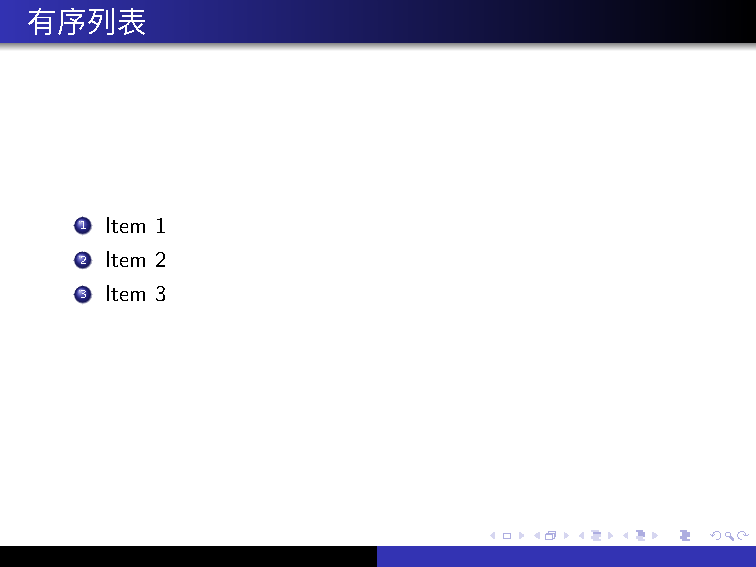
\includegraphics{examples/beamer/beamerlist01.pdf}

\subsection{无序列表}

Unordered lists have a marker, such as a bullet, before every list item. To create an unordered list in beamer, we use the \verb|itemize| environment. Inside this environment, the list entries can be updated using the \verb|\item| command.

A simple unordered list example is presented below.

\inputminted[linenos=true]{latex}{examples/beamer/beamerlist02.tex}

Output:

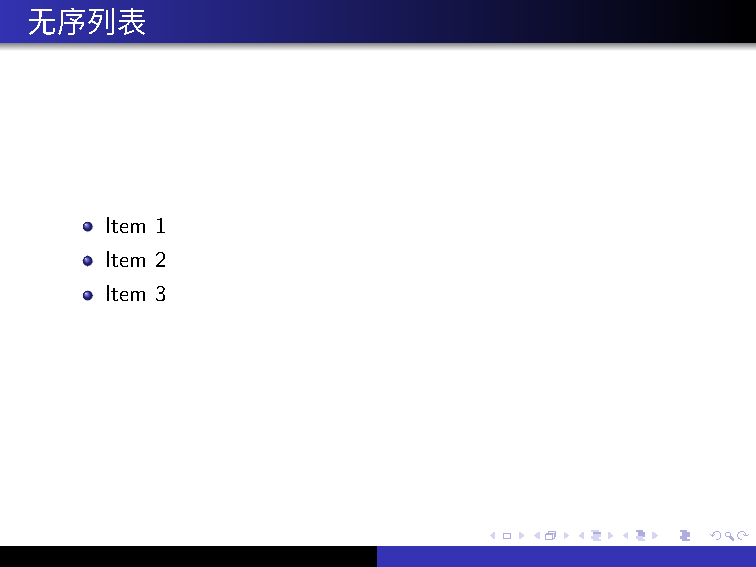
\includegraphics{examples/beamer/beamerlist02.pdf}

\subsection{嵌套列表}

Sometimes you also have to list things, which have some kind of sub-category. For this reason, LaTeX allows you to nest list environments and it will fix the indentation and numbering accordingly.

A simple nested list example is presented below.

\inputminted[linenos=true]{latex}{examples/beamer/beamerlist03.tex}

Compiling this code yields:

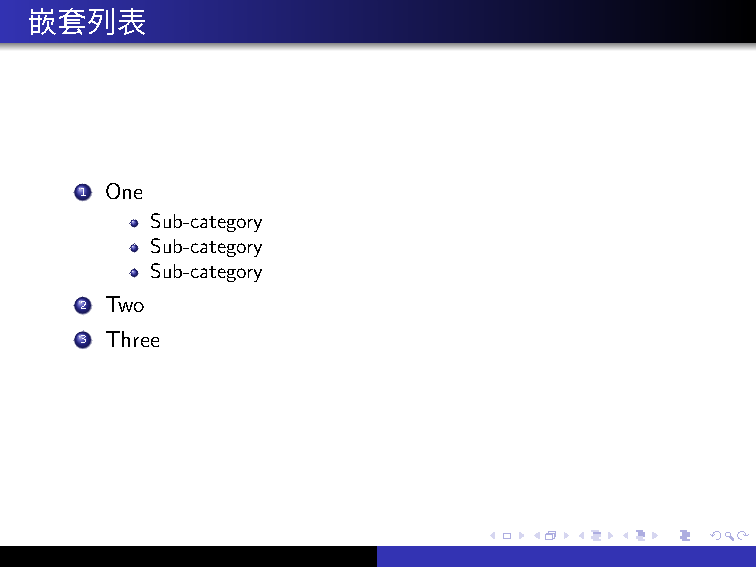
\includegraphics{examples/beamer/beamerlist03.pdf}

\subsection{跨帧列表}

The idea is to define a counter \verb|currentenumi| that stores the value of the last enumerated item in a given frame. Then on the next frame, the \verb|enumi| counter can easily be set to the value of \verb|currentenumi| to continue numbering.

\inputminted[linenos=true]{latex}{examples/beamer/beamerlist04.tex}

which yields the following result:

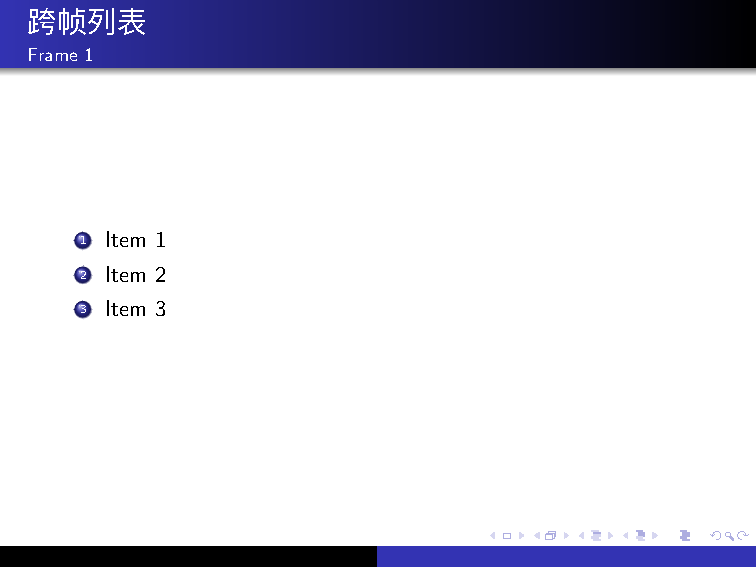
\includegraphics[page=1]{examples/beamer/beamerlist04.pdf}

\includegraphics[page=2]{examples/beamer/beamerlist04.pdf}

\subsection{修改列表项目间距}

The spacing between the list items can be easily altered using the \verb|\vspace| command. The other way to change the spacing globally is to use the following command \verb|\setbeamertemplate|. Here is an illustrative example:

\inputminted[linenos=true]{latex}{examples/beamer/beamerlist05.tex}

Output:

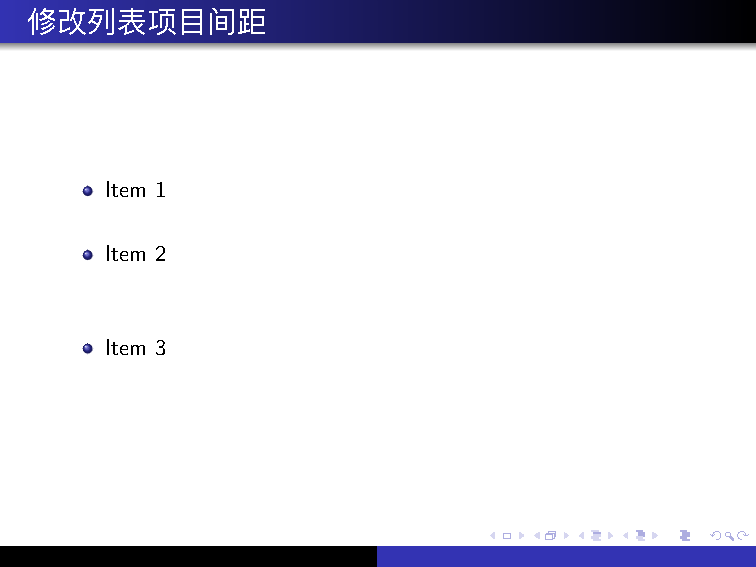
\includegraphics{examples/beamer/beamerlist05.pdf}

Here is another version of spacing between nested lists:

\inputminted[linenos=true]{latex}{examples/beamer/beamerlist06.tex}

Compiling this code yields:

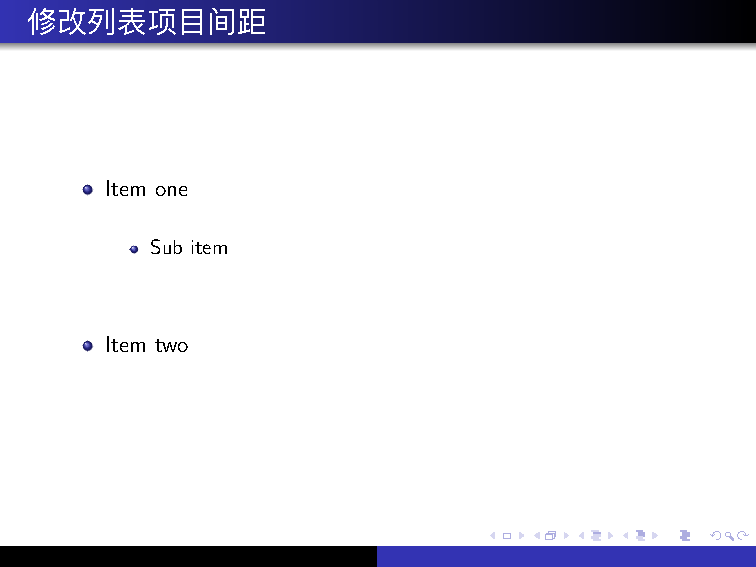
\includegraphics{examples/beamer/beamerlist06.pdf}

\subsection{修改列表项目符号}

There are various templates in beamer to change this itemized list appearance. The command 
\mint{latex}|\setbeamertemplate{itemize itmes}[<shape>]| 
is used on itemize items to change the shape of item markers.

\verb|<shape>| options:

\begin{itemize}
  \item \verb|default| : the default item marker is a triangle.
  \item \verb|circle| : sets the item marker to a small filled circle.
  \item \verb|square| : sets the item marker to a small filled square.
  \item \verb|circle| : sets the item marker to a ball shape.
\end{itemize}

\inputminted[linenos=true]{latex}{examples/beamer/beamerlist07.tex}

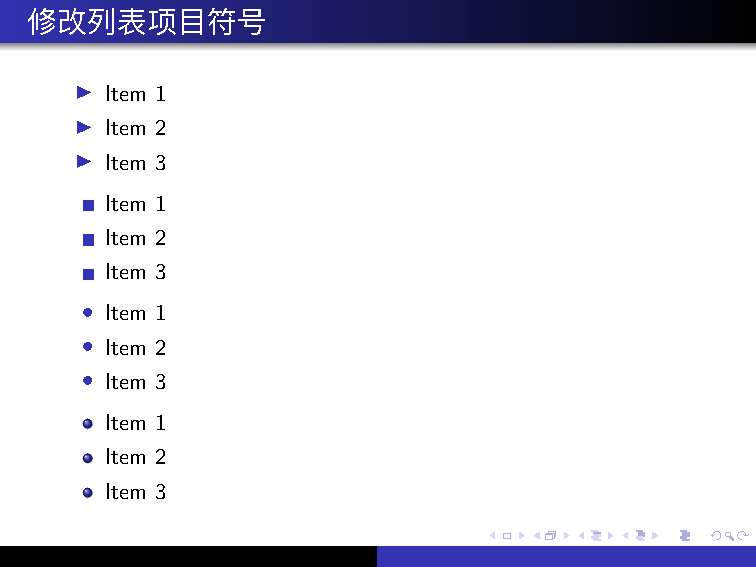
\includegraphics{examples/beamer/beamerlist07.pdf}

使用 pifont 包

\inputminted[linenos=true]{latex}{examples/beamer/beamerlist08.tex}

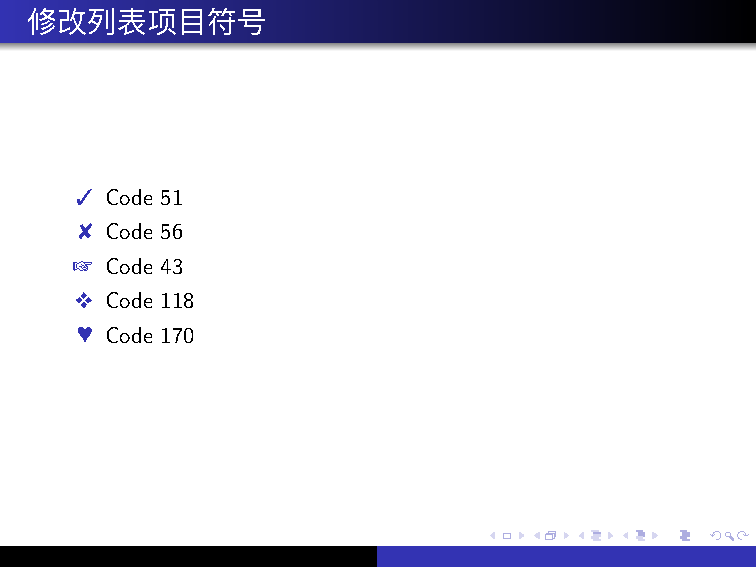
\includegraphics{examples/beamer/beamerlist08.pdf}

\subsection{字母,数字和罗马数字编号}

使用 enumitem 包

Under the enumerate environment, the numbering style can be changed using the enumitem package. From the next example, you can notice that three different styles, alphabet, Roman, and Arabic are used to denote the list item numbers. Meanwhile, you can also separate the enumeration from the item content by enclosing them inside bracket/brackets or a dot.

\inputminted[linenos=true]{latex}{examples/beamer/beamerlist09.tex}

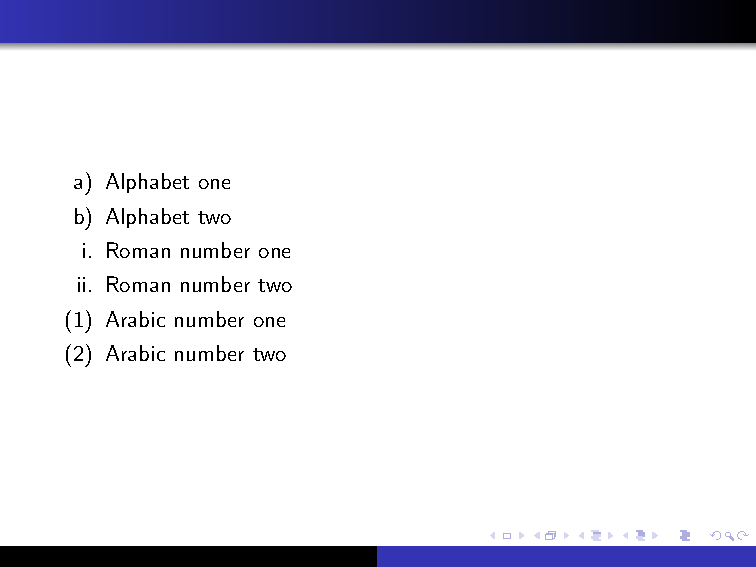
\includegraphics{examples/beamer/beamerlist09.pdf}

% -----------------------------------------------------------------------------
\section{分栏}

\subsection{不同宽度的分栏}

To create columns in beamer, we use the columns environment. Then, at the point to begin a column we use the \verb|\column| command followed by the width of the columns (or {\ttfamily \textbackslash begin\{column\} ...  \textbackslash end\{column\}}).

In the following example, we have created two columns with different widths:

\inputminted[linenos=true]{latex}{examples/beamer/beamercolumn01.tex}

Compiling this code yields:

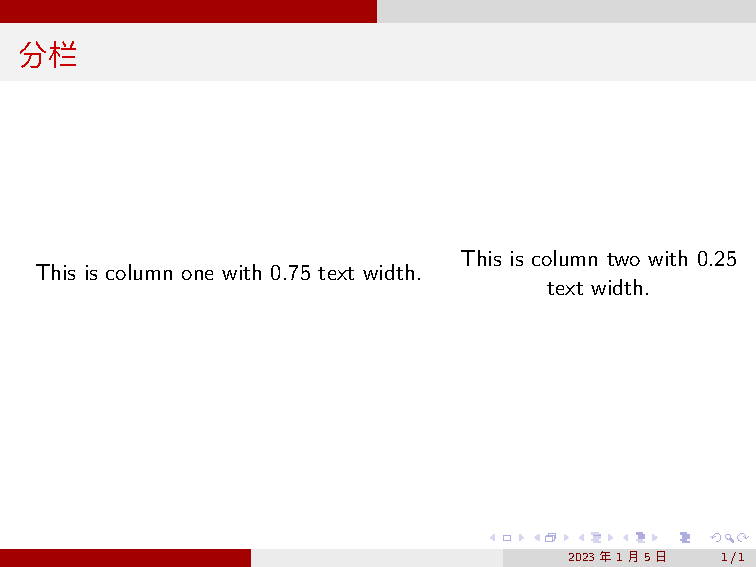
\includegraphics{examples/beamer/beamercolumn01.pdf}

\subsection{文字配图}

With the same manner as above, we can add text and image in the same slide as follows:

\inputminted[linenos=true]{latex}{examples/beamer/beamercolumn02.tex}

Compiling this code yields:

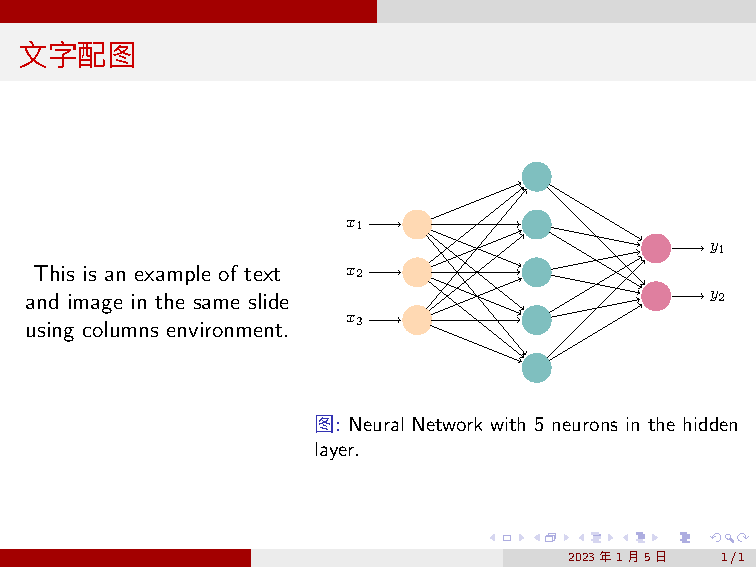
\includegraphics{examples/beamer/beamercolumn02.pdf}

\subsection{垂直分隔线}

To distinctively separate the two (or more) columns from each other we can create a vertical line between them. This can be done simply by adding a \verb|\rule| command in an intermediate column with a small width. In the example below two columns are separated with a vertical line using this method.

\inputminted[linenos=true]{latex}{examples/beamer/beamercolumn03.tex}

Compiling this code yields:

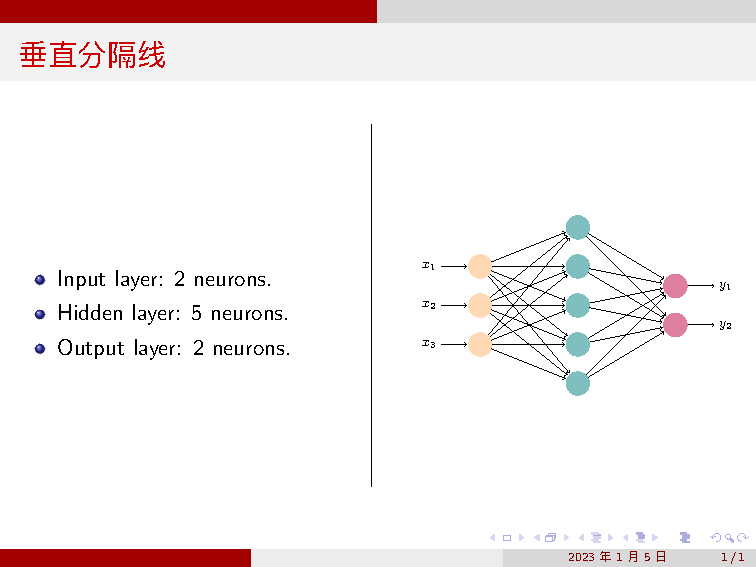
\includegraphics{examples/beamer/beamercolumn03.pdf}

\subsection{垂直方向对齐}

The vertical alignment of column content is very important for the beautification of a presentation. The text and the figures can be placed in three position in a frame, i.e. top, bottom, and center. By specifying [c ], [T], or [b] after beginning the column environment will a automatically position the short content to the center, top, or bottom respectively.

\subsubsection{Top alignment}

\inputminted[linenos=true]{latex}{examples/beamer/beamercolumn04.tex}

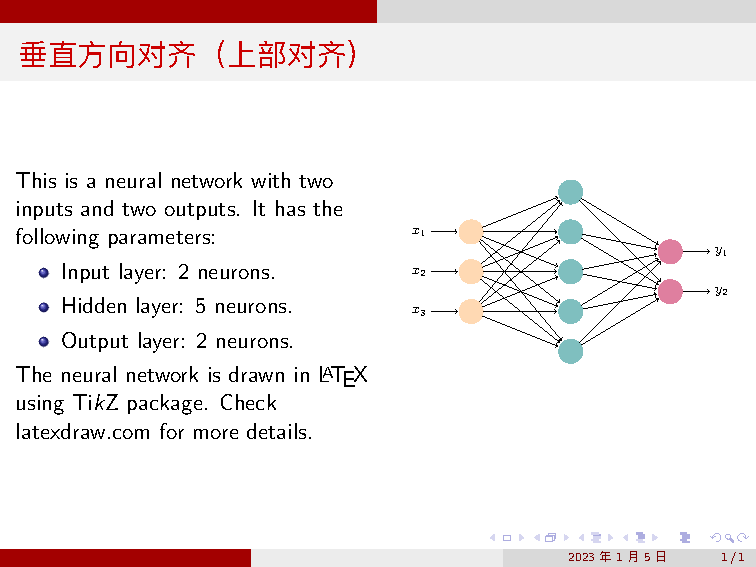
\includegraphics{examples/beamer/beamercolumn04.pdf}

\subsubsection{Center alignment}

\inputminted[linenos=true]{latex}{examples/beamer/beamercolumn05.tex}

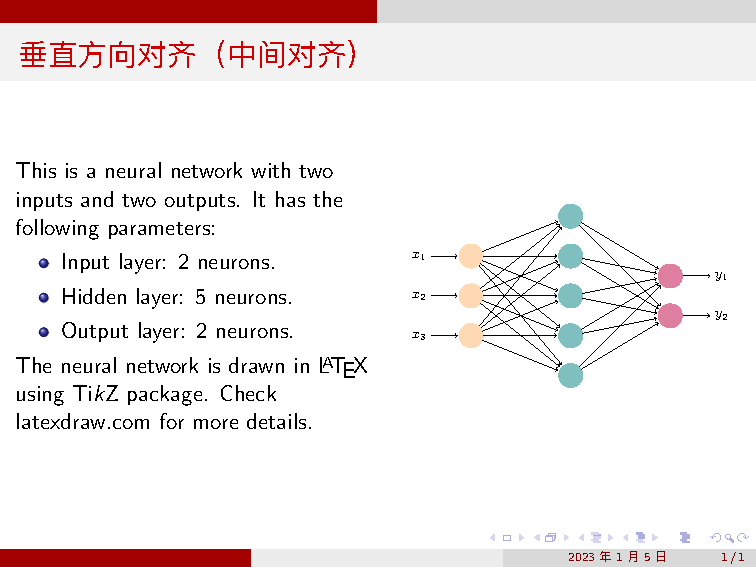
\includegraphics{examples/beamer/beamercolumn05.pdf}

\subsubsection{Bottom alignment}

\inputminted[linenos=true]{latex}{examples/beamer/beamercolumn06.tex}

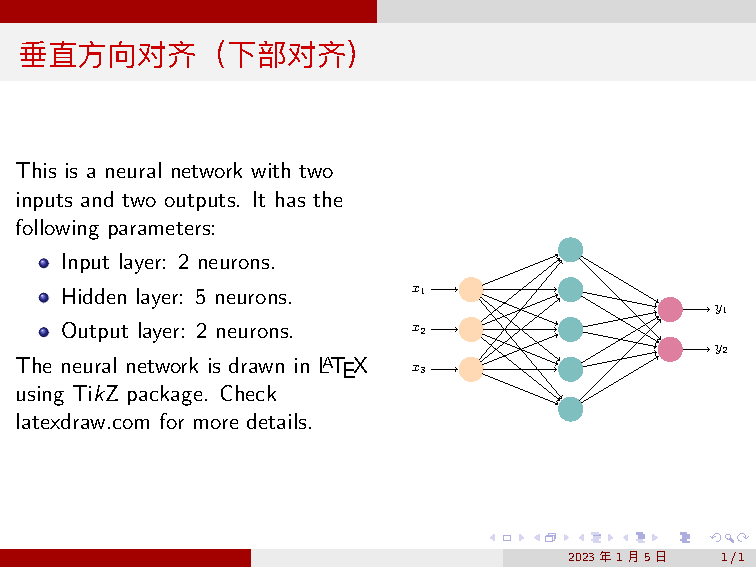
\includegraphics{examples/beamer/beamercolumn06.pdf}

% -----------------------------------------------------------------------------
\section{{\ttfamily block} 环境}

\subsection{创建文字块}

It can be useful to treat some content differently by putting it into a block. In Beamer, we can separate a specific section of text or graphics from the rest of the frame using {\ttfamily block} environment:

\inputminted[linenos=true]{latex}{examples/beamer/beamerblock01.tex}

We used {\ttfamily Madrid} theme for our presentation and inside a frame we added a block environment with title “Block title“. Here is the obtained result:

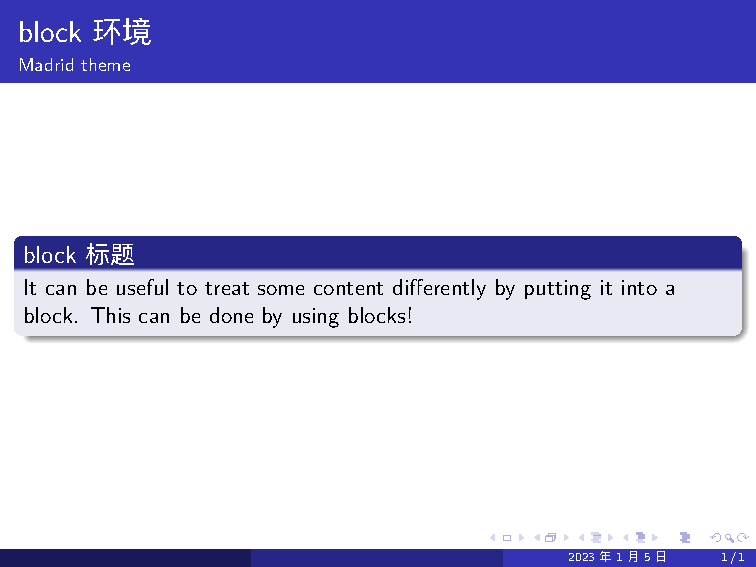
\includegraphics{examples/beamer/beamerblock01.pdf}

It should be noted that the block style depends on the used theme and theme color. Let us consider the same code as above and we change only the them to {\ttfamily Bergen}. The obtained result is shown below:

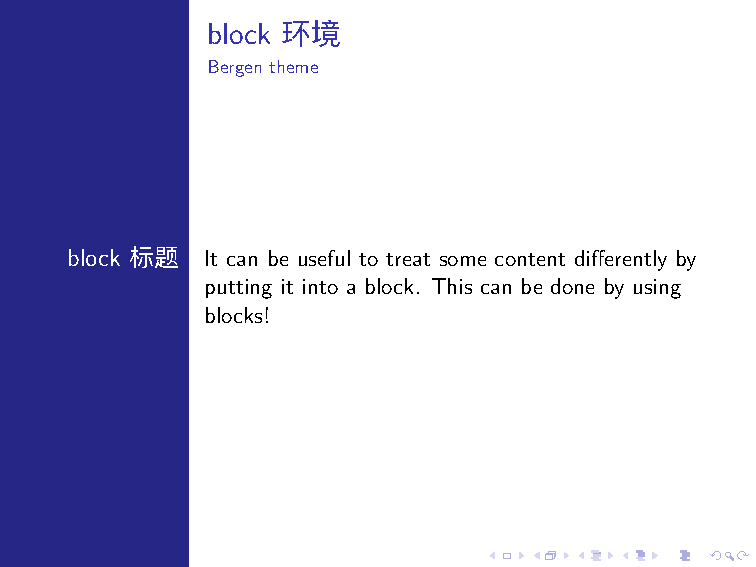
\includegraphics{examples/beamer/beamerblock02.pdf}

\subsection{文字块类型}

There are three basic types of blocks : Standard/Generic block, Alert block, and Example block. There are also special blocks for math environments like Theorem, Definition, Proof, Corollary, Example, etc.

The following table illustrates different blocks with sample code syntax in beamer:

\begin{table}[!h]
\begin{center}
\caption{examples/beamer/Beamer 文字块类型}
\begin{tabular}{cc}
  \toprule
  Content type &  Block\\
  \midrule
  Generic/Standard	& {\ttfamily block}\\
  Highlighted Alert	& {\ttfamily alertblock}\\
  Examples 1	& {\ttfamily exampleblock}\\
  Examples 2	& {\ttfamily example}\\
  Theorems	& {\ttfamily theorem}\\
  Definition	& {\ttfamily definition}\\
  Proofs	& {\ttfamily proof}\\
  Lemmas	& {\ttfamily lemma}\\
  Corollaries	& {\ttfamily corollary}\\
  \bottomrule
\end{tabular}
\end{center}
\end{table}

Here is an example code using different types of blocks in a Beamer presentation:

\inputminted[linenos=true]{latex}{examples/beamer/beamerblock03.tex}

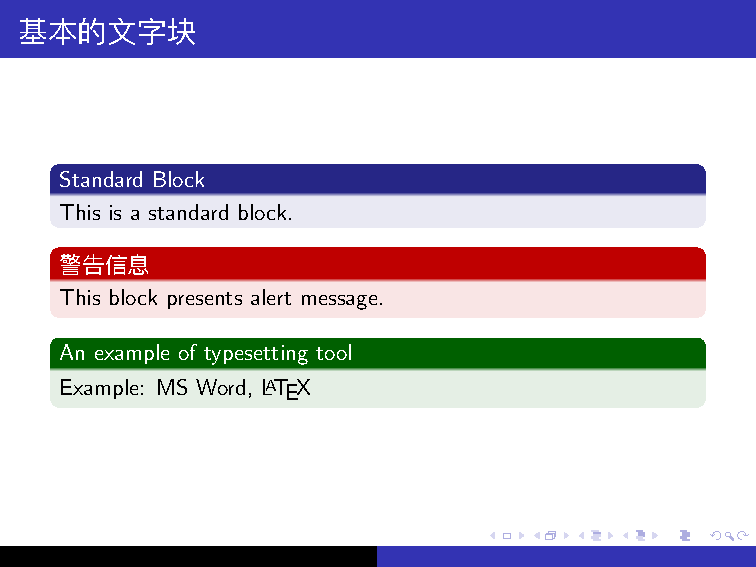
\includegraphics[page=1]{examples/beamer/beamerblock03.pdf}

\includegraphics[page=2]{examples/beamer/beamerblock03.pdf}

\includegraphics[page=3]{examples/beamer/beamerblock03.pdf}

Using {\ttfamily Boadilla} theme instead of {\ttfamily Copenhagen}, we get the following style for different beamer blocks:

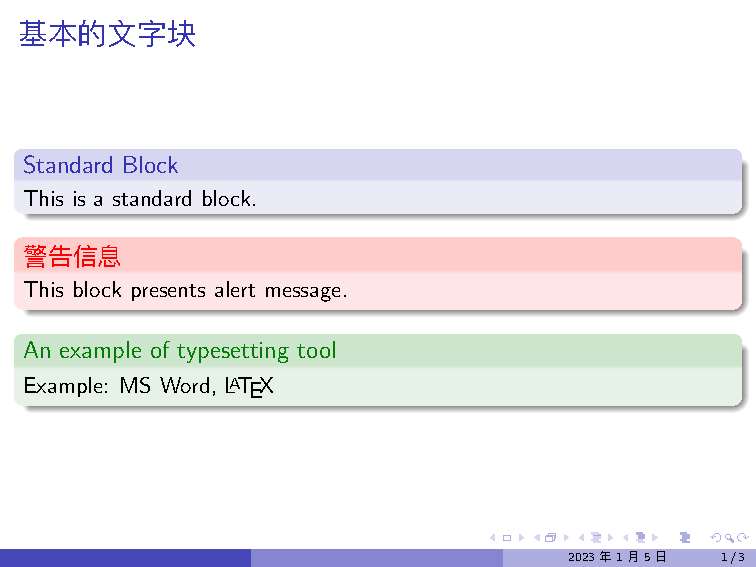
\includegraphics[page=1]{examples/beamer/beamerblock04.pdf}

\includegraphics[page=2]{examples/beamer/beamerblock04.pdf}

\includegraphics[page=3]{examples/beamer/beamerblock04.pdf}

\subsection{自定义文字块}

We can modify blocks’ shapes by playing with the command: 
\mint{latex}|\setbeamertemplate{blocks}[<options>]|
. Here are available pre-defined options for this command:

\begin{itemize}
  \item \verb|default|: This default value typesets the block title on its line.
  \item \verb|rounded|: makes the blocks’ corners rounded.
  \item \verb|shadow=true|: If the shadow is set as true, a shadow is portrayed behind the block.
\end{itemize}

Here is an illustrative example:

\inputminted[linenos=true]{latex}{examples/beamer/beamerblock05.tex}

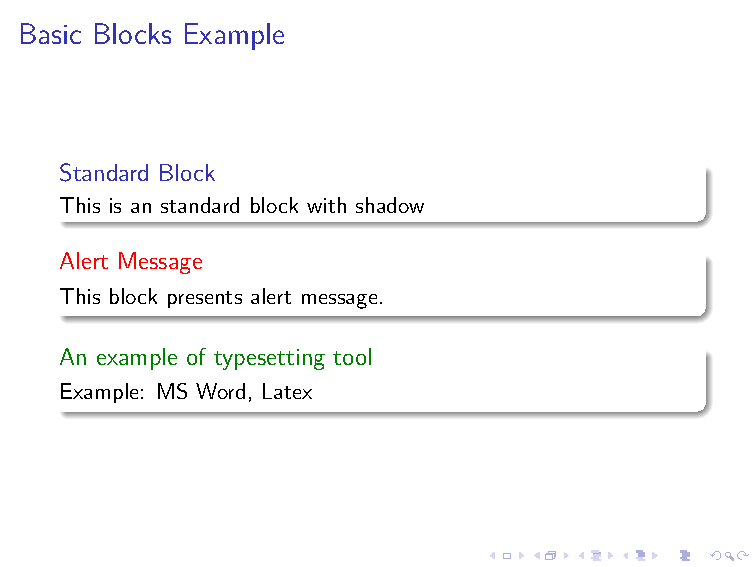
\includegraphics{examples/beamer/beamerblock05.pdf}

\subsection{修改文字块颜色}

From above, we know that blocks’ style depends on the used theme and In this part, we will learn how to change the blocks colors without changing the theme.

For each block (e.g. \verb|alertblock| ), we distinguish two parts: the \verb|title| and the \verb|body| of the block. For each part, we can change the background color and the foreground color. These options can be modified using the command \verb|\{\ttfamily setbeamercolor}|.

In the next example, we changed colors of standard block, alert block and example block. 

\inputminted[linenos=true]{latex}{examples/beamer/beamerblock06.tex}

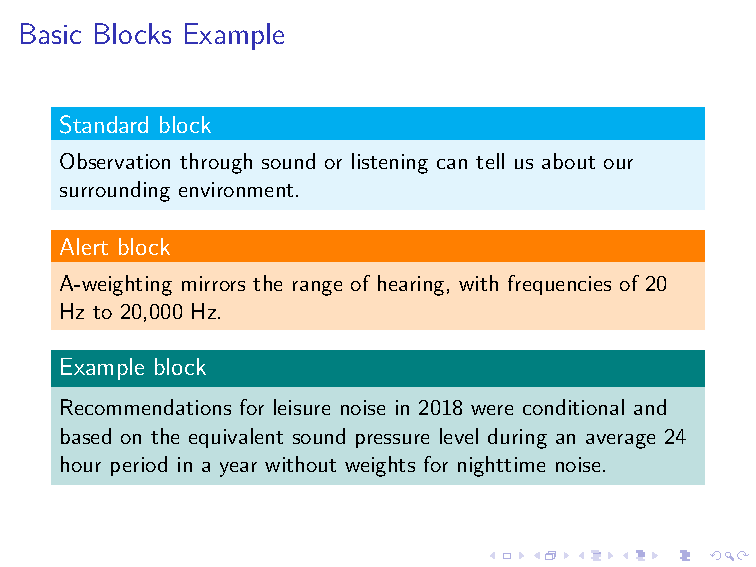
\includegraphics{examples/beamer/beamerblock06.pdf}

% -----------------------------------------------------------------------------
\section{文字格式}

Beamer 中文字格式修饰可以和 {\LaTeX} 其它文档一样,包括粗体、斜体等。
在中文 Beamer 中默认是使用 \verb|\setCJKsansfamily| 定义的字体,
还也可以使用 \verb|\setCJKfamily| 定义中文字体:

\inputminted[linenos=true]{latex}{examples/beamer/beamertextformat01.tex}

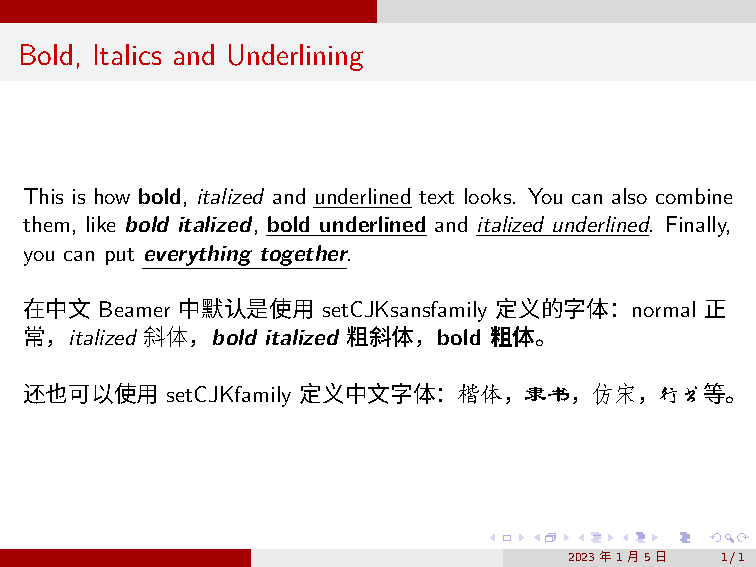
\includegraphics{examples/beamer/beamertextformat01.pdf}

\subsection{Bold Math in Beamer}

As a side note, maybe it is also worth commenting that sometimes we want to use a bold font inside math mode, for instance to denote vectors or matrices. To do so we cannot use the \verb|\textbf| command, but instead we have to load the package bm (which stands for “bold math”) and use the \verb|\bm| command.

\inputminted[linenos=true]{latex}{examples/beamer/beamertextformat02.tex}

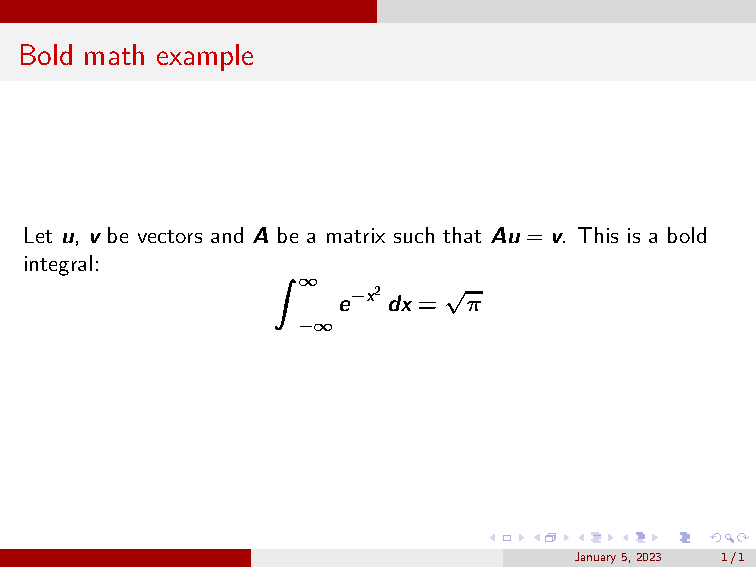
\includegraphics{examples/beamer/beamertextformat02.pdf}

\subsection{Text Decorations in Beamer}

We already saw how to underline text with the \verb|\underline| command that comes with LaTeX. Here we want to go one step further and learn how to do all kinds of “decorations” to our text. To do so, we will be using the ulem package.

This packages mainly changes the way \verb|\emph| works, since instead of emphasizing using the regular italics, it emphasizes the text underlining it. It also introduces the command \verb|\uline| to underline text. By the way, the new underlining is not like the one provided by \verb|\underline|, since the latter will not break at the end of a line, while the former will.

But the ulem package capabilities don’t stop here, since it provides another six more different ways to decorate text.

\begin{table}[!h]
  \begin{center}
  \caption{ulem 宏包命令}
  \begin{tabular}{cc}
    \toprule
    Description	& Command\\
    \midrule
    Underline text solid line	& \verb|\uline|\\
    Double-Underlined text	& \verb|\uuline|\\
    Dashed Underline text	& \verb|\dashuline|\\
    Dotted Underline text	& \verb|\dotuline|\\
    Wavy-Underlined text	& \verb|\uwave|\\
    Strikethrough text	& \verb|\sout|\\
    Struck with Hatching text	& \verb|\xout|\\
    \bottomrule
  \end{tabular}
  \end{center}
\end{table}

对于中文字体修饰可以使用 CJKfntef 宏包,被修饰的文本不要使用 \verb|\CJKfamily| 指定字体,如:\verb|\CJKunderline{{\CJKfamily{楷体}中文}}|。

\inputminted[linenos=true]{latex}{examples/beamer/beamertextformat03.tex}

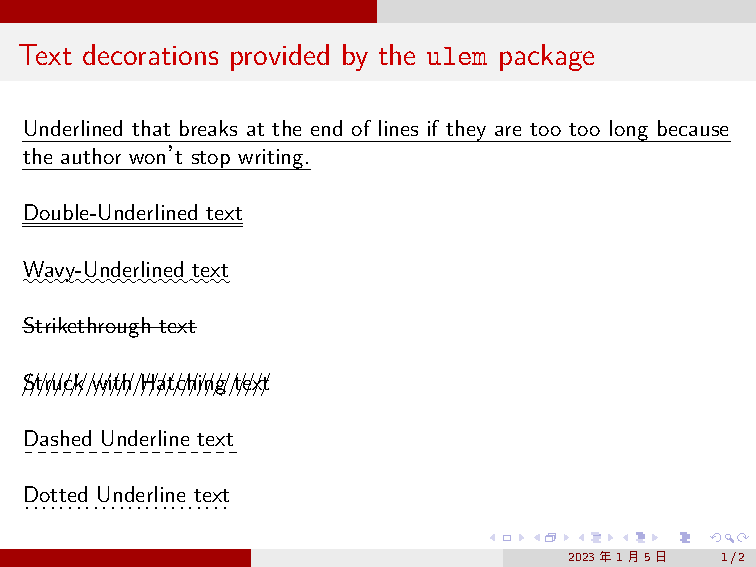
\includegraphics[page=1]{examples/beamer/beamertextformat03.pdf}

\includegraphics[page=2]{examples/beamer/beamertextformat03.pdf}

\subsection{文字对齐}

In general LaTeX documents, paragraphs are usually fully justified, that is, flush both the left and right margins. If you want to change this justification, LaTeX offers the built-in environments flushleft, flushright and center to produce left justified, right justified and centred paragraphs, respectively.

However, there is no built-in environment in LaTeX for fully justified text; and in beamer, by default, the text is left justified. This means that there is no straightforward way of making text fully justified in beamer. This is solved by the ragged2e package, which provides the \verb|\justifying| command. This command, used inside the frame environment, or any other, will produce justified text inside that environment.

The following example shows how to use the different text alignments:

\inputminted[linenos=true]{latex}{examples/beamer/beamertextformat04.tex}

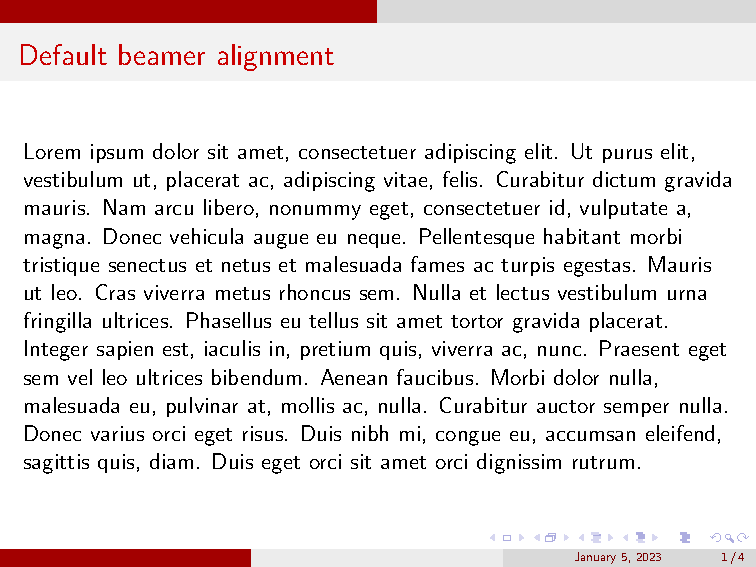
\includegraphics[page=1]{examples/beamer/beamertextformat04.pdf}

\includegraphics[page=2]{examples/beamer/beamertextformat04.pdf}

\includegraphics[page=3]{examples/beamer/beamertextformat04.pdf}

\subsection{调整行距}

If you want to use larger interline spacing in your beamer presentation, you can change its value by using the command:

\verb|\linespread{factor}|

\inputminted[linenos=true]{latex}{examples/beamer/beamertextformat05.tex}

\includegraphics{examples/beamer/beamertextformat05.pdf}

% -----------------------------------------------------------------------------
\section{Beamer 字体}

\subsection{Font Size}

Size is one of the essential properties of a font. The visibility of our content majorly depends on the font size. Predominantly, the Beamer font size was defined in terms of points—for instance, 9 pts, 11 pts, 32 pts, etc .

Beamer has set 11 pts as the normal size of the font. This is the size which is considered as readable from an average distance. Keeping this normal size as datum, other font sizes are defined such as: 
\verb|\tiny|, \verb|\scriptsize|, \verb|\footnotesize|, \verb|\small|, \verb|\normalsize|, \verb|\large|, \verb|\Large|, \verb|\LARGE|, \verb|\huge| and \verb|\Huge|.

The following code highlight different Beamer font size that can be obtained using the above commands:

\inputminted[linenos=true]{latex}{examples/beamer/beamerfont01.tex}

\includegraphics{examples/beamer/beamerfont01.pdf}

Font sizes can also be changed using the beamer class options. We have the sizes: [8pt], [9pt], [10pt], [11pt], [12pt], [14pt], [17pt], [20pt], [bigger], and [small].

Replacing \verb|\documentclass{beamer}| to \verb|\documentclass[14pt]{beamer}|, all font sizes will be shifted where the normal size now is 14pt instead of 11pt. Here is the obtained result:

\includegraphics{examples/beamer/beamerfont02.pdf}

In the process of making our presentation we may face a cramped frame, in which we want to reduce the font size and the line skip, so that all the contents can fit inside. To do so, we can make use of the command

\mint{latex}|\fontsize{<size>}{<vskip>}\selectfont|

Here, and \verb|<vskip>| are TeX dimensions that set the font size and the gap between lines.

This command (as most) will only take effect inside the group or environment in which it is defined; in particular, when put inside a frame environment it will only affect the font sizes of this frame.

Some of the common \verb|<size>| and \verb|<vskip>| units are: point (pt), pica (pc), inch (pt), centimeter (cm) and millimeter (mm).

\begin{minted}{latex}
% Change font size in Beamer
\documentclass{examples/beamer/beamer}

% set a theme
\usetheme{CambridgeUS} 

% Dummy text
\usepackage{lipsum}  

\begin{document}

\begin{frame}{Frame with different font sizes and spacing }{size: 9pt, vskip=10pt}

\fontsize{9pt}{10pt}\selectfont
    
\lipsum[2]
    
\end{frame}
\end{document}
\end{minted}

\subsection{Font Family}

Font family is the second most important property of a Beamer font. Beamer typesets all its text in the \href{https://en.wikipedia.org/wiki/Computer_Modern}{Computer modern} font. There are three types of CM fonts : CM Roman, CM San Serif and CM Typewriter.

Check the following code to get an idea about setting the font family in Beamer:

\inputminted[linenos=true]{latex}{examples/beamer/beamerfont03.tex}

\includegraphics{examples/beamer/beamerfont03.pdf}

We added the option \verb|[fragile]| to be able to use verbatim inside a frame, a more details can be found in \href{https://latex-beamer.com/tutorials/beamer-code/}{“Beamer Code Listing — Syntax highlighter”} lesson.

The other fonts that can be supported by beamer are : Times, Helvetica, Futura.

Besides the font family, beamer has two font series which decide the stroke intensity of the font. The two types of series are : regular and bold. These are obtained using the commands \verb|\mdseries| and \verb|\bfseries|, resepectively.

\subsection{Font Shape and Style}

Beamer supports four types of font shapes: upright, slanted, italics and small caps. Check the example below!

\inputminted[linenos=true]{latex}{examples/beamer/beamerfont04.tex}

\includegraphics{examples/beamer/beamerfont04.pdf}

The upright shape is the default shape for the normal text. The slanted and italics text are seldom used in presentations. The italics font will look same as slant font if the sans-serif font family is used. To have a Times italics effect, the serif font family is mandatory. Italics font shape is used for math. However, the practice of using bold colored text for highlighting is recommended.

The last shape is the small caps. This shape uses smaller versions of the uppercase letters for normal typesetting lowercase letters.

The reading time for the small caps font shape is higher than that for normal text. Thus, making it inadvisable for presentations.

\subsection{Font Weight}

The thickness of the font is referred to as the font weight. The two weights
that are often used are : regular and bold. The bold text is used to create emphasis on a particular topic. The other font weights available in beamer are semibold, ultrabold, thin, and ultrathin.

\subsection{Font Themes}

In this section, we will learn the different pre-defined font themes in beamer. These themes can be used to change the global structure of the presentation.

To change the font family of a theme, we use the command \verb|\usefonttheme| together with one of these font themes:
\begin{itemize}
  \item \verb|default|,
  \item \verb|dserif|,
  \item \verb|dprofessionalfonts|,
  \item \verb|dstructurebold|,
  \item \verb|dstructureitalicserif|,
  \item \verb|dstructuresmallcapsserif|.
\end{itemize}

\subsubsection{Theme font: {\ttfamily default}}

The default font theme installs sans serif font for all text of the presentation and installs different font sizes for elements like titles, headlines and footlines, but does not use boldface or italics for “highlighting.”

Consider the following code that loads the default font theme:

\inputminted[linenos=true]{latex}{examples/beamer/beamerfont05.tex}

\includegraphics[page=1]{examples/beamer/beamerfont05.pdf}

\includegraphics[page=2]{examples/beamer/beamerfont05.pdf}

\subsubsection{Theme font: {\ttfamily professionalfonts}}

Using \verb|\usefonttheme{professionalfonts}| instead of \verb|\usefonttheme{default}| in the above code, we get the following result:

\includegraphics[page=1]{examples/beamer/beamerfont06.pdf}

\includegraphics[page=2]{examples/beamer/beamerfont06.pdf}

\subsubsection{Theme font: {\ttfamily serif}}

This theme causes all text to be typeset using the default serif font.

\includegraphics[page=1]{examples/beamer/beamerfont07.pdf}

\includegraphics[page=2]{examples/beamer/beamerfont07.pdf}

\subsubsection{Theme font: {\ttfamily structurebold}}

This font theme will cause titles and text in the headlines, footlines , and sidebars to be typeset in a bold font.

\includegraphics[page=1]{examples/beamer/beamerfont08.pdf}

\includegraphics[page=2]{examples/beamer/beamerfont08.pdf}

\subsubsection{Theme font: {\ttfamily structureitalicserif}}

This theme is similarly as the structurebold font theme, but where structurebold makes text bold, this theme typesets it in italics and in the
standard serif font.

\includegraphics[page=1]{examples/beamer/beamerfont09.pdf}

\includegraphics[page=2]{examples/beamer/beamerfont09.pdf}

\subsubsection{Theme font: {\ttfamily structuresmallcapsserif}}

Again, this theme does exactly the same as the structurebold font theme, only this time text is set using small caps and a serif font.

\includegraphics[page=1]{examples/beamer/beamerfont10.pdf}

\includegraphics[page=2]{examples/beamer/beamerfont10.pdf}

\subsection{Change Math Font style in Beamer}

To make the math in beamer look like the usual {\LaTeX} math, you only have to insert the following declaration in your preamble \verb|\usefonttheme[onlymath]{serif}|.

The following illustration is obtained with the standard Beamer font:

\includegraphics{examples/beamer/beamerfont11.pdf}

\includegraphics{examples/beamer/beamerfont12.pdf}

% -----------------------------------------------------------------------------
\section{Code Listing in Beamer}

\subsection{{\ttfamily fragile} 选项}

If you try to insert code inside a beamer environment like you would do in any LaTeX document, you will get an error. Whether you type the code using the verbatim, minted or listings environment, since they are all different kinds of verbatim text, you will always get the same error!

To make this environments work, you just have to pass the {\ttfamily fragile} option to the frame where the code will go, and everything will work as expected. 

\subsection{使用 minted 宏包显示代码}

To highlight the use of minted package for code syntax highlighting, we consider the following example:

\inputminted[linenos=true]{latex}{examples/beamer/beamercodelisting01.tex}

\includegraphics{examples/beamer/beamercodelisting01.pdf}

你会发现并没有显示行号,原因在于边距的问题,行号在边距之外。见:

\url{https://tex.stackexchange.com/questions/85105/linenumbers-of-minted-are-not-shown-in-beamer-if-i-use-infolines}

This is caused because the numbers are set in the margin, but with the infolines theme, the margin is too small. It does

\mint{latex}|\setbeamersize{text margin left=1em,text margin right=1em}|

modify to 

\mint{latex}|\setbeamersize{text margin left=1cm,text margin right=1cm}|

\inputminted[linenos=true]{latex}{examples/beamer/beamercodelisting02.tex}

\includegraphics{examples/beamer/beamercodelisting02.pdf}

也可以修改 minted 行号的间隔,见:

\url{https://tex.stackexchange.com/questions/525570/minted-line-numbers-outside-frame-and-outside-margin}

\inputminted[linenos=true]{latex}{examples/beamer/beamercodelisting03.tex}

\includegraphics{examples/beamer/beamercodelisting03.pdf}

\subsection{{\ttfamily fragile} 选项详解}

First of all, we have to understand what {\ttfamily fragile} means. This concept has to do with expansion and execution. {\TeX} does these at the same time: first it reads a token, expands it so that only low-level tokens are left and then executes it. But this cycle isn’t always followed: for instance when moving text around this behavior changes.

For instance, when creating a table of contents, since all the chapters, sections and subsections are scattered around your document, but in the end they all end up in the table of contents. To do so, {\TeX}, when reading and executing a \verb|\section| command, will write the current section’s title and number to a .toc file. After all the commands have been parsed, {\TeX} will fill the table of contents based on the data that was collected in the .toc file.

This can represent a problem because the meaning of code changes during {\TeX}'s process, and only when the typesetting is done the actual meaning of some commands can be determined. So when writing data to a file, some expansions must not occur, because they are dependent on the current situation; examples of these are: commands with optional arguments, line breaks, footnotes and inline math.

To deal with this issues, {\TeX} offers the \verb|\protect| command, which can be used to protect fragile commands. In general, the commands that are not fragile (and thus need not protection) are called robust.

But the real question was why did the frame environment need the fragile option? The beamer user manual tells us that using this option the contents of the frame are written to an external file and then read back.

But again one may ask why bother to do so. The truth is that beamer is a very complex package, to the point that it tunes the {\TeX} internal character codes (which are, in turn, one of the most fundamental elements of {\TeX}). When a frame contains fragile text, different internal mechanisms are used to typeset
the frame to ensure that inside the frame the character codes can be reset.

The price of switching to another internal mechanism is that either you cannot use overlays (one of beamer’s main features, and the reason why character codes are changed, since overlays are specified with the symbols < >, which have to change they character codes) or an external file needs to be written and read back (which is not always desirable, because of the extended compilation time, but is the last option available).

It is clear that the character codes are not easily reset when verbatim code appears inside the frame, since the verbatim environments change the character codes, so that you don’t have to use \{\} as delimiters (and thus you can use them inside the command). For instance, I use the delimiters \verb| |(but to write this, I had to use as delimiters + signs).

% -----------------------------------------------------------------------------
\section{图片}

\subsection{{\ttfamily includegraphics} 命令}

\mint{latex}|\includegraphics{file}|

The above command accepts a series of optional arguments, the most important ones being:\verb|height| and \verb|width| to scale the size of the figure.

When only one of these options is set, the other dimension is scaled so that the aspect ratio of the original image is preserved.

Other less common options are also provided:

\begin{itemize}
  \item \verb|angle| can be passed a rotation angle in degrees, and the image will be rotated this amount counter-clockwise,
  \item \verb|keepaspectratio| is a boolean that forces the image to preserve its aspect ratio.
\end{itemize}

But if you want to do very fancy things, like both rescaling and rotating an image, be aware that the order in which the options are given matters. The package graphicx interprets the keys from left to right; this means that rotating and then scaling is not the same as scaling and then rotating.

Illustrative example:

In the following example, you can see the difference:

\inputminted[linenos=true]{latex}{examples/beamer/beamerfigure01.tex}

which produces:

\includegraphics{examples/beamer/beamerfigure01.pdf}

Observe how the two images are slightly different.

第 1 个图片是先确定宽度再旋转,第 2 个图片是先旋转再确定宽度。

It should be noted that for the width of images we can use a multiple of the text width via the \verb|\textwidth| command. It is very useful when specifying the dimensions of an image since you can set them to a relative amount of width of the text, without having to worry about low-level \verb|TeX| dimensions.

\subsection{设置图片标题}

Although with this we have a totally functional way of inserting images, in practice we don’t insert them this way, since the image has neither a caption nor a way to reference it. It is more convenient to wrap the \verb|\includegraphics| command inside the figure environment. This is a floating environment that lets us set a caption and a label, and also use position specifiers to control where the image will be placed. However, and this is the main point where beamer differs from other {\LaTeX} documents, \textbf{the position specifiers have no effect in beamer presentations}. They are ignored, and the image is simply placed in the same position as in the source code.

Illustrative example:

In the following example, we show how to use the figure environment to insert images:

\inputminted[linenos=true]{latex}{examples/beamer/beamerfigure02.tex}

Compiling this code yields:

\includegraphics{examples/beamer/beamerfigure02.pdf}

Observe that I have added the declaration:

\mint{latex}|\setbeamertemplate{caption}[numbered]|

in the preamble. The reason for this is that, by default, beamer does not number
the pictures (this is another key difference with the usual {\LaTeX} documents), but since I wanted the figure numbered to reference it, I had to change how the caption looks in the beamer template.

Usually, you will not need the number, since every frame will contain one, at most two, images to be explained, and it is not convenient to use numbers as references throughout a presentation (as it is in a document, where you can easily go back and forth).

\subsection{自定义图片标题}

We have already seen how to slightly change the caption appearance, by adding a number to it or not. But we can further customize it by changing its font size and color. The following example shows the beamer theme options that we have to modify in order to customize our caption:

\inputminted[linenos=true]{latex}{examples/beamer/beamerfigure03.tex}

Compiling this code yields:

\includegraphics{examples/beamer/beamerfigure03.pdf}

\subsection{文字与图片分栏}

It is common to write a frame with a figure next to a certain explanation. For this purpose, we can use beamer’s columns environment, as it is done in the following example:

\inputminted[linenos=true]{latex}{examples/beamer/beamerfigure04.tex}

Compiling this code yields:

\includegraphics{examples/beamer/beamerfigure04.pdf}

Observe that the \verb|\textwidth| command in the line:

\mint{latex}|\begin{column}{0.5\textwidth}|

represents the whole text width of the frame, whereas the \verb|\textwidth| in the \verb|\includegraphics| declaration only represents the text width of the column, which is half of the total text width.

This means that, although we pass to the image the option \verb|width=0.7\textwidth|, it doesn’t take 70\% of the frame, but instead, it takes 70\% of the column.

Although in this case, we accompanied the image with text, any kind of content can be used next to it: text, tables, equations, other images, and so on.

\subsection{图片在帧内的对齐}

Almost all of the time we have been using the figure environment to wrap the \verb|\includegraphics| command so that beamer treats the images as floating objects. However, we can also use the raw \verb|\includegraphics| command, and align it using pure TeX filling commands. The reason behind this is that the \verb|\includegraphics| command just creates a {\TeX}’s box with the image inside it; that is, for the TeX system it is just as any other letter.

To easily centre the image, as we have been doing throughout all the tutorial, we can use the \verb|\centering| command just before \verb|\includegraphics|. However, if we want to left-align the image, we will have to use the command \verb|\hfill| just after including the image, so that all the horizontal space after the image is filled by {\TeX}.

Let me show you a complete minimal example of how this would work:

\inputminted[linenos=true]{latex}{examples/beamer/beamerfigure05.tex}

Compiling this code yields:

\includegraphics[page=1]{examples/beamer/beamerfigure05.pdf}

\includegraphics[page=2]{examples/beamer/beamerfigure05.pdf}

And going further we can apply the same principles for the vertical alignment. By default, the image will be vertically centered. However, we can use the \verb|\vfill| command to fill in vertical space, and thus move the image up and down. If we use it before the image, it will be aligned at the bottom, and if we use it after the image, it will be aligned at the top.

\subsection{图片在帧内任意位置}

The following illustration shows different coordinates of a frame that can be used for absolute positioning of an image using TikZ, check this tutorial for more details!

\href{https://latexdraw.com/how-to-create-a-lined-paper-background-in-latex-using-tikz/}{How to Create a Lined Paper Background in LaTeX using TikZ}

\includegraphics[page=1]{examples/beamer/beamer-frame-position.pdf}

Moreover, we can access the frame border using angles as shown below:

\includegraphics[page=2]{examples/beamer/beamer-frame-position.pdf}

The following code highlights the idea of absolute positioning of an image in Beamer using TikZ package:

\inputminted[linenos=true]{latex}{examples/beamer/beamerfigure06.tex}

Comments:

\begin{itemize}
  \item We loaded the TikZ package using the command: \verb|\usepackage{tikz}|
  \item We created a TikZ environment inside a frame that we would like to add an image to it. This is achieved by \verb|tikzpicture| environment.
  \item The parameters of the TikZ environment \verb|[remember picture, overlay]| allows us to work on the frame and use absolute positioning.
  \item We created a node at the center of the frame, (current page.center), which has an image a content.
\end{itemize}

Compiling the above code yields:

\includegraphics[page=1]{examples/beamer/beamerfigure06.pdf}

\includegraphics[page=2]{examples/beamer/beamerfigure06.pdf}

Use left, right, below and above for relative positioning

Now, once you add an image at an absolute position of the frame, you can move it to different directions with respect to the absolute coordinate by adding one of these options: left, right, below or above to the node command!

So to solve the above issue, we can add left option, relative to (current page.east), to the node command.

You can also specify how much left distance by using left=<value> instead of left. 

\inputminted[linenos=true]{latex}{examples/beamer/beamerfigure07.tex}

\includegraphics[page=1]{examples/beamer/beamerfigure07.pdf}

\includegraphics[page=2]{examples/beamer/beamerfigure07.pdf}

You can do the same with right, below and above parameters!

\subsection{修改图片的透明度}

Although we are not going to dive into all of TikZ possibilities, here we are going to explore another functionality that the tikzpicture environment offers: changing the opacity of a figure.

This option is especially interesting when combined with beamer overlay specifications because you can put an image with half its opacity and totally uncover it once you are going to actually talk about it. Even further, you could even decrease the image’s transparency as you get closer to talking about it; this would look very cool.

The following example shows a small implementation of this idea:

\inputminted[linenos=true]{latex}{examples/beamer/beamerfigure08.tex}

\includegraphics[page=1]{examples/beamer/beamerfigure08.pdf}

\includegraphics[page=2]{examples/beamer/beamerfigure08.pdf}

In the above code, we placed the image 1 cm far from the left side of the frame using absolute positioning provided by TikZ. The first version of the image has 30\% opacity and the second one has 100\% opacity.

\subsection{放映设置与图片}

However, if we don’t want such a fancy implementation of opacity, and just want the image to be shown on a given slide, beamer offers us the possibility to pass an overlay specification to the \verb|\includegraphics| command. For example, the declaration:

\mint{latex}|\includegraphics<2-4>[width=\textwidth]{image.png}|

will make the image.png file appear only on slides 2 to 4. 

\subsection{文字环绕图片}

In beamer, we can wrap text around a figure, but not with beamer built-in commands. We have to use the external wrapfig package. In the following example, we use the environment wrapfigure that this package provides to wrap text around a figure:

\inputminted[linenos=true]{latex}{examples/beamer/beamerfigure09.tex}

which produces the following output:

\includegraphics{examples/beamer/beamerfigure09.pdf}

Observe that the {\ttfamily wrapfigure} environment works as the figure environment, in the sense that it makes the image floating, and you can add a \verb|\caption| and a \label to the figure. However, this command accepts two mandatory arguments:

\begin{itemize}
  \item the first one is to select where we want the image, it can be r or l, that is, right or left;
  \item the second one is the width to be reserved for the image.
\end{itemize}

\subsection{文字在图片上}

This can also be done inside a beamer frame, but for that purpose, we have to load the versatile TikZ package. In the following example, we illustrate an easy way to do it:

\inputminted[linenos=true]{latex}{examples/beamer/beamerfigure10.tex}

\includegraphics{examples/beamer/beamerfigure10.pdf}

Let’s dissection the commands used in this example:

\begin{itemize}
  \item First, we insert an image inside the {\ttfamily tikzpicture} environment as a node called ({\ttfamily image}).
  \item Then, we create a second node where its content is aligned at centre, with options to use a white, huge and bold font. Moreover, we added the option {\ttfamily fill=teal} to fill the node with a teal color.
  \item The key is that we position this node at the centre of the previous one; this position is easily identified with {\ttfamily (image.center)}.
  \item Finally, we create the contents of the node itself, which are just the text string {\ttfamily A beautiful photo!}.
\end{itemize}

\subsection{图片作为帧的背景}

nature1.jpg 和 nature2.jpg 来自 \url{https://pixabay.com/}。

It is easy to use an image as a frame background in beamer, both globally and locally. In the following example, we put both into practice:

\inputminted[linenos=true]{latex}{examples/beamer/beamerfigure11.tex}

\includegraphics[page=1]{examples/beamer/beamerfigure11.pdf}

\includegraphics[page=2]{examples/beamer/beamerfigure11.pdf}

You can see that the procedure is very intuitive: we just change the background canvas option of the beamer theme to the image that we want to use as background. However, when importing it we should make sure that the size is adjusted to the frame size; otherwise, we will get undesired results.

\subsection{在 Beamer 中插入子图}

With the subcaption package, we can build floating figure environments that contain more than one image, each with its corresponding caption and label. The following example shows how to do so:

\inputminted[linenos=true]{latex}{examples/beamer/beamerfigure12.tex}

Here is the obtained result:

\includegraphics{examples/beamer/beamerfigure12.pdf}

\begin{itemize}
  \item As you can see, first we create a usual figure environment with its corresponding \verb|\caption| and \verb|\label|.
  \item Then, inside of it, for every subfigure we create a \verb|subfigure| environment, which works essentially as a figure environment, with its corresponding \verb|\includegraphics| to insert the image, its \verb|\caption| and its \verb|\label|.
  \item However, this environment takes a mandatory argument, which is the space to be allocated for the corresponding image (in the previous example, \verb|0.4\textwidth|) and also an optional argument, which determines the positioning of the image inside its allocated space. This argument can be either c, t or b, standing for centre, top and bottom.
  \item By default the image is centred, but in the previous example I have used t and b, so that you can see the difference between the two options.
  \item As you can see, different labels enable us to reference either each one of the subfigures or the figure as a whole.
\end{itemize}

\subsection{图片作为封面}

\subsubsection{Add image to the slide page (bottom)}

The following minimal working example shows how on can include an image in the title page using \verb|\titlegraphics| command:

\inputminted[linenos=true]{latex}{examples/beamer/beamerfigure13.tex}

Compiling this code yields:

\includegraphics{examples/beamer/beamerfigure13.pdf}

It should be noted that titlegraphics content will move the title page details (title, author, institute, etc) to the above. So sometimes we need to fix also the height of the image in the \verb|\includegraphics| command using height=<value> (e.g. \verb|height=0.5\textwidth|).

\subsubsection{Add image to the slide page (top)}

As the title of a presentation is positioned at the top of a title slide, we can include an image just before the title text inside \title{} command:

\inputminted[linenos=true]{latex}{examples/beamer/beamerfigure14.tex}

Compiling this code yields:

\includegraphics{examples/beamer/beamerfigure14.pdf}

% -----------------------------------------------------------------------------
\section{颜色}

There are two ways to change Beamer colors by setting up your own custom color scheme
\footnote{\url{https://ramblingacademic.com/2015/12/08/how-to-quickly-overhaul-beamer-colors/}}. 
The first method is very quick with {\ttfamily usecolortheme}. 
The second method takes a little bit of tinkering with {\ttfamily setbeamercolor}, but ultimately gives you much more control.

\subsection{Picking Beamer Colors}

The first decision is to pick a color(s). I suggest defining two colors for variety, where one is your primary and one is your secondary. However, only one color is needed for the {\ttfamily usecolortheme} method. There are two ways to pick colors:

\begin{itemize}
  \item Choose from the list of known Beamer colors. By default, Beamer uses the xcolor package, so you can immediately use any of xcolor‘s pre-defined colors. As of this writing, these colors are listed in Section 2.4 of the official xcolor documentation. For example, the list includes blue, red, green, yellow, etc. A list of 68 colors is available if you load xcolor with the {\ttfamily dvipsnames} option when you load Beamer ({\ttfamily documentclass[xcolor=dvipsnames]\{beamer\}}).
  \item Define your own custom colors. Use the {\ttfamily definecolor} command to assign a custom name and then define the parameters for your color (such as RGB values). This is handy if you want to use a very specific color, as I did.
\end{itemize}

\section{使用 {\ttfamily usecolortheme} 命令修改 Beamer 颜色}

The command {\ttfamily usecolortheme} can be used to load any of the default Beamer color themes (as displayed on \url{https://www.hartwork.org/beamer-theme-matrix/}). 
But this post is about not using the default color themes. You can use {\ttfamily usecolortheme} with any color you want by applying the color to the {\ttfamily structure} of the presentation.

\mint{latex}|{\ttfamily usecolortheme}[named=UBCblue]{structure}|

Here is a minimal example. I’ve chosen to use the Madrid theme with the {\ttfamily miniframes} outer theme (to add a header) and the {\ttfamily circles} inner theme (to replace the shiny default circles).

\inputminted[linenos=true]{latex}{examples/beamer/beamercolor01.tex}

Compiling this code yields:

\includegraphics[page=1]{examples/beamer/beamercolor01.pdf}

\includegraphics[page=2]{examples/beamer/beamercolor01.pdf}

\section{使用 {\ttfamily setbeamercolor} 命令修改 Beamer 颜色}

If you just want a break from the default color themes, then {\ttfamily usecolortheme} is sufficient. If you want to define exactly what colors are used, then a little more work is required (but not much). My goal was to use UBC’s official colors, so a better solution was needed.

A key find was Thierry Masson’s \href{http://www.cpt.univ-mrs.fr/~masson/latex/Beamer-appearance-cheat-sheet.pdf}{Beamer appearance cheat sheet}. This document lists many of the properties that you can manipulate. Page 1 of the sheet lists things that you can color using {\ttfamily setbeamercolor}. You can play around with it, but here is a quick method to color your entire presentation:

\begin{itemize}
  \item Set the background color of ALL FOUR palettes to your primary color. Set the foreground color of each palette to your desired text color (most likely black or white).
  \item Set the color of elements that are not defined by the palettes. You can use your primary or secondary color. This might be the hardest step and could take some trial and error to catch everything. The most important one is {\ttfamily structure} (for bullets and numbers in lists). If you have a table of contents, then you will also want to set {\ttfamily section} in {\ttfamily toc}. Anything you don’t catch will appear in the default colour theme.
  \item (optional) Select some palette elements where you would like to see the secondary color and set the color for just those elements. For example, setting {\ttfamily subsection} in {\ttfamily head/foot} to the secondary color has a nice clean appearance in themes that use a header or footer. Why not set a whole palette to the secondary color? You can, but I’ve found that you can end up with some undesirable results in headers.
\end{itemize}

\inputminted[linenos=true]{latex}{examples/beamer/beamercolor02.tex}

Compiling this code yields:

\includegraphics[page=1]{examples/beamer/beamercolor02.pdf}

\includegraphics[page=2]{examples/beamer/beamercolor02.pdf}

% -----------------------------------------------------------------------------
\section{超链接与按钮}

\subsection{超链接{\ttfamily \textbackslash hyperlink}}

首先使用 \verb|\label| 命令标记需要链接的地方,然后使用

\mint{latex}|\hyperlink{<label>}{<text>}|
插入超链接:

\inputminted[linenos=true]{latex}{examples/beamer/beamerhyperlink01.tex}

\includegraphics[page=1]{examples/beamer/beamerhyperlink01.pdf}

\includegraphics[page=2]{examples/beamer/beamerhyperlink01.pdf}

\subsection{按钮}

按钮和超链接是类似的:

\begin{minted}{latex}
\hyperlink{<label>}{\beamerbutton{<text>}}
\hyperlink{<label>}{\beamergotobutton{<text>}}
\hyperlink{<label>}{\beamerskipbutton{<text>}}
\hyperlink{<label>}{\beamerreturnbutton{<text>}}
\end{minted}

\includegraphics[page=2]{examples/beamer/beamerhyperlink02.pdf}

% -----------------------------------------------------------------------------
\section{Beamer 主题}

\subsection{Standard Beamer themes}

Beamer comes with a large selection of themes. Themes are named after various cities, such as Boadilla, Madrid, Copenhagen, and Singapore, where Beamer’s author and his collaborators have given Beamer presentations.

Beamer themes which are named after cities, such as Boadilla and Pittsburgh, are complete themes in the sense that they control just about every aspect of a slide’s appearance. Think of these as major themes. These are invoked with the \verb|\usetheme| command, as in {\ttfamily \textbackslash usetheme\{Pittsburgh\}}.

Beamer also provides what may be thought of as minor themes. These control somewhat narrowly defined aspects of a slide’s appearance. You may invoke one or more of these minor themes in conjunction with a major theme to alter/modify the major theme’s characteristics.

Beamer’s “minor themes” fall into 4 categories: outer, inner, font and color themes.

default 主题

\inputminted[linenos=true]{latex}{examples/beamer/beamertheme01.tex}

\includegraphics{examples/beamer/beamertheme01.pdf}

Boadilla 主题

\includegraphics{examples/beamer/beamertheme02.pdf}

Rochester 主题

\mint{latex}|\usetheme[height=7mm]{Rochester}|

修改标题栏的高度

\includegraphics{examples/beamer/beamertheme03.pdf}

\subsection{outer themes}

control a slide’s decorations, such as text and graphics that appear in a slide’s header and footer sections. For example, {\ttfamily \textbackslash useoutertheme \{shadow\}} adds a 3-D shadow to some header elements.

\subsection{inner themes}

control a slide’s inner area, such as markers/bullets for itemization lists and boxes placed around theorems. For example, {\ttfamily \textbackslash useinnertheme \{rounded\}} gives a rounded and 3-D look to theorem-containing boxes and itemization markers.

\subsection{font themes}

control font shapes and sizes of various elements of a slide show. For example, {\ttfamily \textbackslash usefonttheme \{serif\}} changes the document’s fonts to serif. (The default is sans-serif.)

\subsection{color themes}

control the colors of title, frame title, itemization bullets, and many other elements of a slide show. For example, {\ttfamily \textbackslash usecolortheme \{albatross\}} changes the Beamer’s default colors in quite a drastic way.

% -----------------------------------------------------------------------------
\section{自定义主题}

\subsection{{\ttfamily structure} 颜色}

\begin{remark*} 
  下面的代码会产生{\ttfamily Package xcolor: Undefined color `beamer@structure@color'}错误:
  \mint{latex}|\documentclass[xcolor=dvipsnames]{beamer}|
  应该使用:
  \mint{latex}|\documentclass[dvipsnames]{beamer}|

  下面的代码会产生产生 {\ttfamily LaTeX Error: Option clash for package xcolor.} 错误:
  \mint{latex}|\usepackege[dvipsnames]{xcolor}| 
  This above syntax may result in an error if you are using beamer with tikz. To go around it, include usenames and dvipsnames options when defining the document class. 见\url{https://en.wikibooks.org/wiki/LaTeX/Colors#The_68_standard_colors_known_to_dvips}
  \mint{latex}|\documentclass[usenames,dvipsnames]{beamer}|

  其它解决方法:使用 \verb|\definecolor| 自定义颜色;如果要使用 hex 值定义颜色,则使用不带选项的 xcolor 包,如:
  \mint{latex}|\definecolor{BlueGreen}{HTML}{00B3B8}|
\end{remark*}



\inputminted[linenos=true]{latex}{examples/beamer/beamertheme04.tex}

\includegraphics{examples/beamer/beamertheme04.pdf}

通过 RGB 值设置颜色

\mint{latex}|\usecolortheme[RGB={205,173,0}]{structure}| 

\subsection{删除导航图标}

\inputminted[linenos=true]{latex}{examples/beamer/beamertheme05.tex}

\includegraphics{examples/beamer/beamertheme05.pdf}

\subsection{添加底部信息栏}

\inputminted[linenos=true]{latex}{examples/beamer/beamertheme06.tex}

\includegraphics{examples/beamer/beamertheme06.pdf}

\subsection{修改默认文本颜色}

Beamer’s normal text is black on white background. The following command in the preamble changes all normal text to purple:

\mint{latex}|\setbeamercolor{normal text}{fg=purple}|

\inputminted[linenos=true]{latex}{examples/beamer/beamertheme07.tex}

\includegraphics{examples/beamer/beamertheme07.pdf}

The fg in command above sets the normal text’s foreground color. It is also possible to set the normal text’s background color. The background color of a slide is inherited from the normal text’s background, therefore changing the normal text’s background color amounts to changing the slide’s background color. See  Setting the background to a solid color for an illustration.

Remark: Normal text is the text in the main body of a slide. A slide’s header and footer are not normal text. The colors of those elements are controlled by the structure color. For instance, the following command changes slide titles (and several other things) to purple:

\mint{latex}|\setbeamercolor{structure}{fg=purple}| 

\subsection{修改背景颜色}

The background color of a Beamer slide is white by default. In the following example I will describe a few ways to change the default background.


Setting the background to a solid color

This example shows how to set the background to a light shade of pink:

\inputminted[linenos=true]{latex}{examples/beamer/beamertheme08.tex}

\includegraphics{examples/beamer/beamertheme08.pdf}

\subsection{背景颜色渐变}

Gradually shaded backgrounds are possible as well. In the following example, the background varies from light red at the bottom to light yellow at the top.

\inputminted[linenos=true]{latex}{examples/beamer/beamertheme09.tex}

\includegraphics{examples/beamer/beamertheme09.pdf}

\subsection{背景图片}

The following example shows how to fill the background of a Beamer slide with the scaled version of an image using the command:

\mint{latex}|\setbeamertemplate{background canvas}{...}|

Note how I have changed the structure color and the default font color to achieve a reasonable contrast between text and background.

\inputminted[linenos=true]{latex}{examples/beamer/beamertheme10.tex}

\includegraphics{examples/beamer/beamertheme10.pdf}

\subsection{背景图片的透明度}

通过 tikz 绘图来设置图片的透明度:

\inputminted[linenos=true]{latex}{examples/beamer/beamertheme11.tex}

\includegraphics{examples/beamer/beamertheme11.pdf}

\subsection{限制背景设置在单个帧}

To limit the background setting to a single slide, enclose the 

\mint{latex}|\setbeamertemplate{background canvas}{...}|
command in braces, as in:

\begin{minted}{latex}
{ % brace to limit the scope of \setbeamertemplate 
\setbeamertemplate{navigation symbols}{}  % optionally hide navigation buttons 
\setbeamertemplate{background canvas}{\includegraphics 
	[width=\paperwidth,height=\paperheight]{alps.jpg}} 
\begin{frame}[plain] 
... 
\end{frame} 
} % closing brace 
\end{minted}

\includegraphics[page=1]{examples/beamer/beamertheme12.pdf}

\includegraphics[page=2]{examples/beamer/beamertheme12.pdf}

% -----------------------------------------------------------------------------
\section{创建自己的 Beamer 主题}

参考实例:

\begin{itemize}
  \item Metropolis theme \url{https://github.com/matze/mtheme}
  \item Bruno theme \url{https://forge.delab.re/matteo/beamertheme-bruno}
  \item THK theme \url{https://github.com/Markus-de-Koster/LaTeX-beamer-TH-Koeln}
  \item Amurmaple theme \url{https://plmlab.math.cnrs.fr/mchupin/mcbeamertheme}
  \item SINTEF theme \url{https://www.overleaf.com/latex/templates/sintef-presentation/jhbhdffczpnx}
  \item Lucid theme \url{https://www.overleaf.com/latex/examples/building-a-custom-beamer-theme/hkbgktmpjckz}
  \item Beamer Templates \url{https://latex-beamer.com/beamer-template/}
\end{itemize}

According to the guide, Beamer presentations have five flavours of themes

\begin{itemize}
  \item Presentation themes – Every aspect of the presentation is detailed here. The colour, the font, the way the bullets look. The way the enumeration goes. The size and position of the logo etc.
  \item Colour themes – Just of the colour details. This can be created as a separate file from the presentation theme and then later called with other presentation themes. I will explain this below. In fact, let’s just enumerate the other three and jump to the explanation of how all this connects.
  \item Font themes
  \item Inner themes – Design the elements that are “inside” the frame like the environments, theorems, blocks etc.
  \item Outer themes – Design the outer space of the frame like the headline, footline, sidebar etc. 
\end{itemize}

修改 Beamer 首页的背景方法\footnote{\href{https://latex-beamer.com/tutorials/beautiful-title/}{How to create beautiful title slide in Beamer?}}:

\inputminted[linenos=true]{latex}{examples/beamer/themes/background/beautiful-title.tex}

我们可以修改上面的代码得到一个简单的 Beamer 主题,能够设定 Beamer 背景图片:

\inputminted[linenos=true]{latex}{examples/beamer/themes/background/beamerthemenovel.sty}

使用该主题的示例:

\includegraphics[page=1]{examples/beamer/themes/background/sample01.pdf}

\includegraphics[page=1]{examples/beamer/themes/background/sample02.pdf}

% -----------------------------------------------------------------------------
\section{覆盖 Overlay}

\subsection{{\ttfamily \textbackslash pause} 命令}

Often when when doing a presentation we'll want to reveal parts of a frame one after the other. The simplest way to do this is to use the \verb|\pause| command. For example, by entering the \verb|\pause| command before every entry in a list we can reveal the list point-by-point:

\inputminted[linenos=true]{latex}{examples/beamer/beameroverlay01.tex}

This brings us on to the difference between a frame and a slide. A single frame is defined as what we build up in a single frame environment, whereas a slide is a single page in the resulting PDF. This means that a frame can be made up of multiple slides. For example, this frame with the list that we've just animated is made up of five slides, but the frame number in the bottom-right-hand corner of each slide remains unchanged for all of the five.
The fully exposed slide looks like this:

\includegraphics[page=5]{examples/beamer/beameroverlay01.pdf}

The use of the \verb|\pause| command is not restricted to itemized lists; you may use it anywhere in a slide. For example:

\inputminted[linenos=true]{latex}{examples/beamer/beameroverlay02.tex}

A pdf viewer will expose the resulting file one paragraph at a time. The fully exposed slide looks like this:

\includegraphics[page=4]{examples/beamer/beameroverlay02.pdf}

\subsection{覆盖说明 Overlay specifications}

The \verb|\pause| command is useful but isn't very versatile. To get more flexibility we use what beamer calls overlay specifications. These specifications can be added to compatible commands using pointed brackets after the command name. For example I can add them to the \verb|\item| command in a list structure like this.

\inputminted[linenos=true]{latex}{examples/beamer/beameroverlay03.tex}

The numbers inside the pointed brackets tell LaTeX which slides the item should appear on. For example, in this list we've told each list item which slide number it should first appear on and then told them to appear on all subsequent slides in the frame using the dash. Here's an example of a more complicated overlay:

\mint{latex}|\item<-2,4-5,7>|

This makes the item appear on slides 1,2,4,5 \& 7.

\includegraphics[page=1]{examples/beamer/beameroverlay03.pdf}

There are a number of commands that enable us to use overlays on text. The main one is the \verb|\onslide| command which can be configured to achieve a few different outcomes, details of these can be found in the \href{http://mirrors.ctan.org/macros/latex/contrib/beamer/doc/beameruserguide.pdf}{documentation}.

\inputminted[linenos=true]{latex}{examples/beamer/beameroverlay04.tex}

When we simply give this command text as an argument, it acts in the same way as the \verb|\uncover| command making the text fully appear only on the specified slides. On unspecified slides the text is covered, so will still take up space but won't be visible.

\includegraphics[page=1]{examples/beamer/beameroverlay04.pdf}

\includegraphics[page=2]{examples/beamer/beameroverlay04.pdf}

\includegraphics[page=3]{examples/beamer/beameroverlay04.pdf}

To make the text transparent on unspecified slides we use the \verb|\setbeamercovered| command and enter the keyword transparent above the code where we want it to have an effect:

\mint{latex}|\setbeamercovered{transparent}|

\includegraphics[page=1]{examples/beamer/beameroverlay05.pdf}

\includegraphics[page=2]{examples/beamer/beameroverlay05.pdf}

\includegraphics[page=3]{examples/beamer/beameroverlay05.pdf}

Please be aware that this command will affect all of the code following it, so if we want to change it back to the default setting later in the presentation we can simply use the same command again but with the keyword invisible.

Another command we can use is the \verb|\visible| command which does the same as \verb|\uncover| except it leaves the space blank on unspecified slides instead of transparent even if we've set the transparency as we did a moment ago.

The \verb|\invisble| command does the exact opposite to of the \verb|\visible| command. The \verb|\only| command does the same as the \verb|\visible| command except it doesn't take any space up. This means that if we change the \verb|\onslide| commands to \verb|\only| commands and get rid of the dashes in the overlay specifications our three lines of text will appear in the same place on the frame in turn.

\inputminted[linenos=true]{latex}{examples/beamer/beameroverlay06.tex}

\includegraphics[page=1]{examples/beamer/beameroverlay06.pdf}

\includegraphics[page=2]{examples/beamer/beameroverlay06.pdf}

\includegraphics[page=3]{examples/beamer/beameroverlay06.pdf}

\subsection{Overlays and text formatting}

There are a number of commands to do with text formatting that are compatible with overlay specifications. These commands are simply ignored on slides not declared in the specification and will therefore just print the text as normal. Here are some examples:

\inputminted[linenos=true]{latex}{examples/beamer/beameroverlay07.tex}

Which will produce text like this on the first slide:

\includegraphics[page=1]{examples/beamer/beameroverlay07.pdf}

And then like this on the second slide:

\includegraphics[page=2]{examples/beamer/beameroverlay07.pdf}

First the \verb|\textbf| command which makes the text bold, then \verb|\textit| which puts the text in italics, then \verb|\textsl| which make it slanted, \verb|\textrm| which uses the roman font family, \verb|\textsf| which uses the sans serif font family but this doesn't change anything because we are already using this font. Next the \verb|\textcolor| command which puts it in the specified colour, then \verb|\alert| which puts the text in red by default and finally the \verb|\structure| command which formats the text in a way that indicates the presentation's structure.

\subsection{Overlays and environments}

Overlay specifications often work with environments as well. For example, we could animate the environments on the maths blocks page like this:

\inputminted[linenos=true]{latex}{examples/beamer/beameroverlay08.tex}

\includegraphics[page=1]{examples/beamer/beameroverlay08.pdf}

\includegraphics[page=2]{examples/beamer/beameroverlay08.pdf}

You will also notice that turning the transparency setting on earlier in the document has affected the overlays here.

\subsection{Overlays and tables}

Finally we may want to animate a table so that the rows appear slide by slide. To do this we use the \verb|\onslide| command and make sure we reset the \verb|\setbeamercovered| command to the default for this to work:

\inputminted[linenos=true]{latex}{examples/beamer/beameroverlay09.tex}

\includegraphics[page=1]{examples/beamer/beameroverlay09.pdf}

\includegraphics[page=2]{examples/beamer/beameroverlay09.pdf}

% -----------------------------------------------------------------------------
\section{分发 Handout}

Now let's briefly look at creating handouts for our presentation. To do this we add the keyword \verb|handout| into square brackets in the document class command. We then use the pgfpages package to help us print multiple slides on a page. After loading the package we use the \verb|\pgfpagesuselayout| command. In the curly brackets we specify how many frames we want on a sheet. In the square brackets we specify the paper size and how much border shrink we want:

\begin{minted}{latex}
\documentclass[handout]{beamer}
\usepackage{pgfpages}
\pgfpagesuselayout{2 on 1}[a4paper,border shrink=5mm]
\end{minted}

If we wanted to put four frames on a sheet we could simply change the 2 to a 4 and then add the landscape keyword into the square brackets:

\mint{latex}|\pgfpagesuselayout{4 on 1}[a4paper,border shrink=5mm,landscape]|

This concludes our discussion on themes and handouts and also our series on creating presentations with beamer. If you want to play around with the presentation we created in this series you can access it here.

\includegraphics[page=1,scale=.45]{examples/beamer/handout/pythagorean-theorem.pdf}

\includegraphics[page=2,scale=.45]{examples/beamer/handout/pythagorean-theorem.pdf}